%% Ceci est un exemple et un gabarit pour les articles publi{\'e}s par la 
%% Revue Ouverte d'Intelligence Artificielle (ROIA)

%% �La classe cedram.cls et son option cedram-ROIA.clo doivent se
%% trouver dans le r{\'e}pertoire de pr{\'e}paration de l'article, ou dans le
%% chemin de recherche de LaTeX.  Elle est bas{\'e}e sur la classe 
%% amsart.cls (version 2) et impl{\'e}mente la mise en page de la revue,
%% ainsi que quelques commandes sp{\'e}cifiques en vue de la mise en ligne.  
%% Les options disponibles : 
%% francais pour les articles {\'e}crits en fran{\c c}ais 
%% (anglais n'est pas n{\'e}cessaire car c'est la langue par d{\'e}faut). 
%% Unicode pour disposer des caract{\`e}res accentu{\'e}s sans avoir recours {\`a}
%% des macros (ceci impose un codage utf8). 
%% L'option manuscript est obligatoire pour les manuscrits pr{\'e}par{\'e}s
%% par les auteurs.
\documentclass[francais,ROIA,Unicode,manuscript]{cedram}

%% On peut charger ici des extensions standard si les fonctions
%% fournies sont n{\'e}cessaires {\`a} la compilation de l'article. 
%\usepackage[matrix,arrow,tips,curve]{xy}
% \usepackage{gensymb}
% \usepackage{booktabs}
% \usepackage{algorithmic}
% \usepackage[french,onelanguage,linesnumbered,algoruled]{algorithm2e}
% ...
\usepackage{subcaption}
\usepackage{xcolor}
% --- Tickz
\usepackage{physics}
\usepackage{tikz}
\usepackage{amsmath}
\usepackage{mathdots}
% \usepackage{yhmath}
\usepackage{cancel}
\usepackage{color}
\usepackage{siunitx}
\usepackage{array}
\usepackage{multirow}
% \usepackage{amssymb}
\usepackage{gensymb}
\usepackage{tabularx}
\usepackage{extarrows}
\usepackage{booktabs}
\usetikzlibrary{fadings}
\usetikzlibrary{patterns}
\usetikzlibrary{shadows.blur}
\usetikzlibrary{shapes}
% ---------

\usepackage[inline, shortlabels]{enumitem}
\usepackage{arydshln}
\usepackage{amssymb}
\usepackage{csquotes}
\usepackage[export]{adjustbox}

\usepackage{tabularray}\UseTblrLibrary{varwidth}
\usepackage{xcolor}
\def\BibTeX{{\rm B\kern-.05em{\sc i\kern-.025em b}\kern-.08em
    T\kern-.1667em\lower.7ex\hbox{E}\kern-.125emX}}
\usepackage{amsmath}
\newcommand{\probP}{\text{I\kern-0.15em P}}

\newcommand{\myCustomSize}[1]{%
  \fontsize{9}{10.8}\selectfont
  #1
}

\DeclareMathAlphabet\mathbfcal{OMS}{cmsy}{b}{n}

\usepackage{amssymb}
\usepackage{pifont}

\newcommand{\cmark}{\ding{51}}
\newcommand{\xmark}{\ding{55}}

\addto\extrasfrench{%
\renewcommand{\figureautorefname}{Figure}
% \renewcommand{\lstlistingautorefname}{Listing}
\renewcommand{\tableautorefname}{Table}
\renewcommand{\partautorefname}{Partie}
\renewcommand{\appendixautorefname}{Appendice}
\renewcommand{\chapterautorefname}{Chapitre}
\renewcommand{\sectionautorefname}{Section}
\renewcommand{\subsectionautorefname}{Sous-section}
}

%% D{\'e}finitions utilisateur et macros pratiques...  De telles
%% d{\'e}finitions sont interdites dans les titres, les r{\'e}sum{\'e}s ou la
%% bibliographie.
%\newcommand{\la}{\longrightarrow}
% ...

%% Un ensemble de th{\'e}or{\`e}mes sont pr{\'e}d{\'e}finis. La r{\`e}gle mn{\'e}motechnique
%% est que le nom de l'environnement est form{\'e} des quatre premi{\`e}res
%% lettres (sans accents) de l'{\'e}tiquette utilis{\'e}e (theo, exam, rema,
%% coro, conj, etc.) ; les versions ast{\'e}risqu{\'e}es (non num{\'e}rot{\'e}es)
%% existent de m{\^e}me (theo*, etc.). Pour ne pas modifier vos habitudes
%% de saisie, il est possible de d{\'e}clarer, par exemple :
%\equalenv{remark}{rema}
%% qui d{\'e}finit un environnement � remark � identique {\`a} � rema �.

%% Le titre de l'article: syntaxe d'amsart.
\title
%% L'argument optionnel donne la version courte pour les ent{\^e}tes.
%% Inutile si le titre est suffisamment court 
[MOISE+MARL]
%% L'argument obligatoire est imprim{\'e} sur la premi{\`e}re page, dans les
%% ent{\^e}tes si la version courte n'est pas sp{\'e}cifi{\'e}e.
{MOISE+MARL : un cadre organisationnel pour l’explicabilité et le contrôle en apprentissage par renforcement multi-agent \textsuperscript{(1)}}

%% The English title of the article.
\alttitle{MOISE+MARL: an organizational framework for explainability and control in multi-agent reinforcement learning}

%% Les noms des auteurs, selon la syntaxe d'amsart, avec en outre la
%% distinction pr{\'e}nom/nom
\author{\firstname{Julien} \lastname{Soulé}}
\address{Université Grenoble Alpes, Grenoble INP, LCIS, 26000 Valence, France}
\author{\firstname{Michel} \lastname{Occello}} 
\address[2]{Grenoble Alpes University, LCIS, 26000 Valence, France}
\author{\firstname{Jean-Paul} \lastname{Jamont}} 
\address[2]{Université Grenoble Alpes, Grenoble INP, LCIS, 26000 Valence, France}
\author{\firstname{Louis-Marie} \lastname{Traonouez}} 
\address[3]{Thales Land and Air Systems, BU IAS, 35000 Rennes, France}
\author{\firstname{Paul} \lastname{Théron}} 
\address[4]{AICA IWG, 26000 Valence, France}

%Mickaël Bettinelli$^{1}$, Michel Occello$^{1}$ and Damien Genthial$^{1}$

%% N'inclure aucune autre information dans l'argument de la macro
%% \author ! Toutes les autres donn{\'e}es ont des commandes sp{\'e}cifiques :



%% Addresse de messagerie {\'e}lectronique
\email{julien.soule@lcis.grenoble-inp.fr}


%% Les cr{\'e}dits ou remerciements ne se mettent pas en note dans
%% \author, mais {\`a} part :
%\thanks{L'auteur a b{\'e}n{\'e}fici{\'e} d'un soutien important de la communaut{\'e}.}

%% En pr{\'e}sence de coauteurs, chacun est saisi ici de la m{\^e}me fa{\c c}on,
%% dans l'ordre alphab{\'e}tique.
%\author{\firstname{Alan} \middlename{W.} \lastname{Turing}}
%\address{Big Apple University\\
% Myself Institute \\
%  Wilmslow, UK}
%\email{turing@turing.edu.uk}

%% Mots et expressions cl{\'e}s :
\keywords{Apprentissage par renforcement multi-agent, Système Multi-Agent, Explicabilité, Contrôle, Organisation}
  
%% Mots et expressions cl{\'e}s en anglais :
\altkeywords{Multi-Agent Reinforcement Learning, Multi-Agent System, Explainability, Control, Organization}

% %% Mots et expressions cl{\'e}s en espagnol :
% \keywordsES{Muy similarez,  igual-fatal , Maquina M{\'\i} a}


%% R{\'e}sum{\'e}
\begin{abstract}
Des agents en apprentissage par renforcement multi-agent peuvent développer des comportements interprétables comme des rôles ou objectifs implicites, suggérant une hypothétique organisation émergente. Afin d’exploiter pleinement cette analogie, nous introduisons MOISE+MARL, un cadre organisationnel qui couple le modèle organisationnel $\mathcal{M}OISE^+$ à un modèle Markovien afin d’améliorer le contrôle et l’explicabilité des politiques apprises.
MOISE+MARL guide ou contraint les agents selon des rôles et des objectifs en ajustant dynamiquement leurs actions et récompenses, et intègre une méthode d’analyse permettant d’inférer a posteriori des spécifications organisationnelles implicites à partir des trajectoires des agents.
MOISE+MARL a été évalué sur quatre environnements et plusieurs algorithmes d'apprentissage par renforcement multi-agent. Les résultats montrent que les politiques des agents convergent plus rapidement, sont plus stables et deviennent plus explicables. La méthode d'analyse est confirmé par la cohérence entre les spécifications organisationnelles définies et celles inférées.
\end{abstract}

%% R{\'e}sum{\'e} anglaisss
\begin{altabstract}
Multi-agent reinforcement learning agents can develop interpretable behaviors such as implicit roles or objectives, suggesting a hypothetical emergent organization. To fully exploit this analogy, we introduce \textsc{MOISE+MARL}, an organizational framework that couples the organizational model $\mathcal{M}OISE^+$ with a Markovian model in order to improve both the control and the explainability of the learned policies.  
\textsc{MOISE+MARL} guides or constrains agents through roles and objectives by dynamically adjusting their actions and rewards, and integrates an analysis method that allows inferring implicit organizational specifications \textit{a posteriori} from the agents’ trajectories.  
\textsc{MOISE+MARL} was evaluated on four environments and several multi-agent reinforcement learning algorithms. The results show that agents’ policies converge faster, are more stable, and become more explainable. The analysis method is validated by the consistency between the predefined organizational specifications and the inferred ones.
\end{altabstract}

%%�R{\'e}sum{\'e} espagnol
% \begin{abstractES}
%  Eso es el Resumen.
% \end{abstractES}

%% Toutes ces informations doivent se trouver avant \maketitle, et
%% encore mieux : avant \begin{document}

\begin{document}

\maketitle


\section{Introduction}

% Contexte
\noindent
L'apprentissage par renforcement multi-agent~\cite{maisonhaute2024} (\textit{Multi-Agent Reinforcement Learning -- MARL}) constitue aujourd'hui un paradigme central pour l'entraînement d'agents constituant un Système Multi-Agent (SMA). Il vise à déterminer une \emph{politique conjointe} qui régit simultanément les actions individuelles des agents ainsi que leurs interactions, de manière à atteindre un objectif collectif sans qu'il soit nécessaire de spécifier explicitement les mécanismes de coordination~\cite{Albrecht2024book}.
%
Cette axe de recherche a démontré son intérêt dans de nombreux domaines tels que la robotique collective~\cite{Wang2025}, la gestion de ressources distribuées~\cite{Chahoud2025} ou la cybersécurité~\cite{Hammar2023}.

\noindent
Dans des environnements nécessitant une forte composante d'interactions sociales, il n’est pas rare que les agents convergent vers des comportements collectifs réguliers. Ces comportements peuvent être interprétés comme la manifestation implicite de \textbf{rôles} (c’est-à-dire des fonctions assumées spontanément par certains agents) et de la poursuite coordonnée d’\textbf{objectifs}, ce qui peut donner l’impression de l’émergence d’une organisation~\cite{Foerster2016}.
%
Cette dynamique rapproche partiellement ces systèmes d’une véritable \textbf{organisation multi-agent}, structurée et fonctionnelle, similaire à celles décrites par des cadres normatifs comme AGR~\cite{ferber2003} (\textit{Agent Group Roles}) ou $\mathcal{M}OISE^+$~\cite{Hubner2007}. Dans ces modèles, les spécifications organisationnelles, comme les rôles ou objectifs, constituent les briques fondamentales pour décrire le comportement attendu d’un SMA. La comparaison entre comportements émergents du MARL et organisation explicite suggère ainsi un rapprochement entre apprentissage et modèle organisationnel.

% Problématique
\noindent
Toutefois, l’identification fiable de ces rôles et objectifs émergents demeure une tâche complexe. En effet, en émettant l'hypothèse que tout agent MARL suit une politique retranscrite par un rôle et des objectifs implicites possiblement inconnus, les comportements d'agents entraînés peuvent fréquemment apparaître comme \emph{bruités}, \emph{irréguliers} ou dépendants de dynamiques locales difficiles à interpréter. Cette variabilité rend délicate toute tentative de caractériser, de manière systématique, les régularités collectives comme de véritables \emph{rôles} ou \emph{objectifs}.
%
Pour capturer cette difficulté, nous introduisons la notion d’\textbf{adéquation organisationnelle}. Ce concept est théorisé comme la proximité entre les comportements appris par les agents par rapport aux comportements produits par des agents suivant une organisation explicite et normative. En cherchant à déterminer et à maîtriser dans quelle mesure les politiques apprises respectent ou s’écartent des spécifications organisationnelles définies, l'adéquation organisationnelle ouvre alors la voie à une double problématique encore peu explorée dans le domaine du MARL : le \textbf{contrôle} et l’\textbf{explicabilité}.
%
\begin{itemize}
    \item \textbf{Évaluation de l’adéquation organisationnelle.}
          Il s’agit de mesurer l’alignement d’une politique conjointe avec une organisation explicitement définie, c’est-à-dire un ensemble de comportements réguliers attendus. Or, la littérature existante reste principalement centrée sur l’inférence ou l’assignation de rôles~\cite{Isakov2024, Wen2024, Xie2024} au sein et pour le bénéfice de l'apprentissage seulement.

    \item \textbf{Contrôle de l’adéquation organisationnelle.}
          Il consiste à orienter l’apprentissage des agents vers des politiques conformes à une organisation cible, au moyen de \emph{contraintes} ou \emph{incitations} explicites. Un tel contrôle permet non seulement de réduire l’espace de recherche des politiques, mais aussi d’améliorer la convergence des algorithmes et d’assurer le respect de contraintes de sûreté ou de sécurité.
\end{itemize}


% Contribution
\noindent Nous présentons le cadre \textbf{MOISE+MARL} qui articule une double contribution :
%
\begin{itemize}
    \item \textbf{Unification MARL et modèle organisationnel : }
          MOISE+MARL combine la structure du modèle Markovien Dec-POMDP (\textit{Decentralized Partially Observable Markov Decision Process}) avec le modèle organisationnel $\mathcal{M}OISE^+$, afin de spécifier la logique des rôles et objectifs. Le cadre permet alors d'appliquer des rôles et objectifs aux agents, en ajustant leurs actions et leurs récompenses pour favoriser / imposer l’alignement organisationnel.
    \item \textbf{Méthode d'analyse organisationnelle : }
          MOISE+MARL comprend la méthode TEMM (\textit{Trajectory-based Evaluation in MOISE+MARL}) qui propose un mécanisme d’analyse \emph{a posteriori} permettant d’inférer automatiquement des rôles et objectifs à partir des trajectoires d’agents. En mobilisant des techniques d’apprentissage non supervisé, cette méthode fournit une mesure quantitative de l’\emph{adéquation organisationnelle}.
\end{itemize}

\noindent Contrairement au \textit{Hierarchical Reinforcement Learning} (HRL)~\cite{Qi2024,Matsuyama2025}, qui repose sur une décomposition interne des tâches, MOISE+MARL applique le guidage/contrainte organisationnelle avec un ensemble limité de spécifications organisationnelles, de façon \emph{externe} et indépendante de l'apprentissage, favorisant l’\emph{utilisabilité} et la \emph{scalabilité}.

% Évaluation et résultats
\noindent
Nous avons évalué MOISE+MARL selon trois axes principaux :
%
\begin{itemize}
    \item \textbf{Diversité des environnements} : Quatre environnements MARL ont été sélectionnés, chacun nécessitant des formes d’organisation implicite différentes, afin de tester la généralisabilité du cadre à des contextes variés ;
    \item \textbf{Multiplicité des algorithmes} : Quatre algorithmes MARL issus des familles \textit{policy-based}, \textit{actor-critic} et \textit{value-based} ont été comparées avec les spécifications organisationnelles durant l’apprentissage et l’analyse post-entraînement ;
    \item \textbf{Spécifications organisationnelles dédiées} : Pour chaque environnement, un ensemble de rôles, objectifs et permissions/obligations a été défini, permettant une évaluation manuelle ou via TEMM de l’impact organisationnel sur les politiques apprises.
\end{itemize}
%
Bien que l’établissement des spécifications organisationnelles nécessite un investissement initial, leur application permet généralement d’accélérer la convergence et de stabiliser les politiques apprises. Cela atténue le problème de non-stationnarité et contribue également à résoudre partiellement le problème d’attribution du mérite, qui sont des difficultés inhérentes au MARL~\cite{Albrecht2024book}.
L’analyse manuelle montre que les agents dotés de rôles et d'objectifs adoptent des comportements conformes aux spécifications organisationnelles. Les rôles et objectifs inférés par TEMM correspondent aux spécifications prédéfinies, validant la cohérence interne du cadre.  Enfin, il est à noter que les algorithmes basés sur la politique et acteur-critique semblent produire des politiques plus stables que les algorithmes basés sur la valeur.

% Structure de l'article  
\noindent La \autoref{sec:related_works} examine les travaux liés à l'adéquation organisationnelle, la \autoref{sec:moise_marl_framework} détaille le cadre MOISE+MARL, la \autoref{sec:TEMM_algorithm} présente la méthode TEMM, la \autoref{sec:experimental_setup} décrit le protocole expérimental, la \autoref{sec:results} analyse les résultats obtenus, et enfin la \autoref{sec:discussion_conclusion_future_work} propose une conclusion et des perspectives.

\section{Travaux connexes}
\label{sec:related_works}

Cette section explore des travaux liant l'organisation avec le MARL.

\subsection{Évaluation de l'adéquation organisationnelle}

L'évaluation de l'adéquation organisationnelle consiste à vérifier si les comportements acquis par les agents correspondent à une organisation explicitement définie ou émergente. Les principaux critères considérés sont :
(E1) l’identification des rôles implicites,
(E2) la détection des objectifs et missions atteints,
(E3) la cohérence structurelle,
(E4) la mesure quantitative de l’adéquation organisationnelle,
et (E5) l’explicabilité des comportements collectifs.
%
Nous présentons ici les travaux saillants liés au sujet de l'inférence de rôles ou d'objectifs afin d'évaluer l'adéquation organisationnelle ou des notions proches.

Des mécanisme de découverte et de transfert de rôles à travers différents environnements ont été proposées pour identifier des rôles implicite~\cite{wilson2008learning}. Toutefois, ces rôles sont définis comme des abstractions statistiques internes à l’apprentissage, et ne permettent pas de satisfaire les critères de \emph{cohérence structurelle} ou de \emph{mesure explicite de l’adéquation organisationnelle}. L’explicabilité reste limitée à l’interprétation des structures de rôles transférées

Yusuf et Baber~\cite{yusuf2020inferential} contribue indirectement à la \emph{cohérence structurelle} en gérant l’incertitude et les conflits entre agents par inférence bayésienne. Toutefois, elle ne vise ni l’\emph{identification de rôles implicites}, ni la \emph{détection explicite d’objectifs ou missions}. L’absence de métriques quantitatives d’adéquation organisationnelle et de représentations interprétables limite sa portée au regard des critères recherchés.

Dans le cadre de missions \textit{Unmanned Aerial Vehicle}, une approche a été proposée pour montrer que les agents apprennent à coordonner leurs actions et ressources pour coopérer efficacement~\cite{berenji2000learning}. Cependant, l’approche ne formalise pas la notion de \emph{rôle implicite} généralisable et n’évalue pas la \emph{cohérence structurelle} au sein d’une organisation. La mesure d’adéquation est absente, et l’explicabilité reste limitée à des scénarios de coopération spécifiques.

Serrino et al.~\cite{serrino2019finding} propose d'aborder l’\emph{identification de rôles implicites}, mais uniquement sous la forme de relations sociales locales (allié/adversaire). Cela contribue à l’explicabilité immédiate des interactions, mais ne satisfait pas les critères de \emph{cohérence structurelle}, de \emph{mesure d’adéquation organisationnelle} ou de \emph{détection de missions globales}. L’évaluation reste contextuelle et ne s’appuie pas sur une organisation normative.

\medskip
\noindent
En résumé, les travaux identifiés couvrent partiellement certains critères en particulier l’identification de rôles~\cite{serrino2019finding,wilson2008learning}, la détection d’objectifs dans des missions spécifiques~\cite{berenji2000learning} mais aucun ne répond simultanément à l’ensemble des critères recherchés, laissant un vide que nous souhaitons combler comme illustré dans la \autoref{tab:evaluation_criteria_summary}.

\begin{table*}[h!]
    \centering
    \caption{Travaux liés à l’évaluation de l’adéquation organisationnelle}
    \label{tab:evaluation_criteria_summary}
    \renewcommand{\arraystretch}{1.3}
    \scriptsize
    \begin{tabular}{
        p{3cm}
        >{\centering\arraybackslash}p{1.4cm}
        >{\centering\arraybackslash}p{1.4cm}
        >{\centering\arraybackslash}p{1.4cm}
        >{\centering\arraybackslash}p{1.4cm}
        >{\centering\arraybackslash}p{1.4cm}
        }
        \hline
        \textbf{Travaux}                                      & \textbf{(E1) Identification de rôles} & \textbf{(E2) Détection objectifs / missions} & \textbf{(E3) Cohérence structurelle} & \textbf{(E4) Mesure quantitative} & \textbf{(E5) Explicabilité organisationnelle} \\ \hline
        Wilson et al. (2008)~\cite{wilson2008learning}        & \checkmark                            & $\times$                                     & $\times$                             & $\times$                          & $\sim$                                        \\
        Berenji \& Vengerov (2000)~\cite{berenji2000learning} & $\times$                              & \checkmark                                   & $\times$                             & $\times$                          & $\sim$                                        \\
        Yusuf \& Baber (2020)~\cite{yusuf2020inferential}     & $\times$                              & $\times$                                     & $\sim$                               & $\times$                          & $\times$                                      \\
        Serrino et al. (2019)~\cite{serrino2019finding}       & \checkmark                            & $\times$                                     & $\times$                             & $\times$                          & $\sim$                                        \\
        Wang et al. (2020)~\cite{wang2020roma}                & \checkmark                            & $\times$                                     & $\sim$                               & $\times$                          & $\sim$                                        \\
        Nguyen et al. (2022)~\cite{nguyen2022transfer}        & \checkmark                            & $\sim$                                       & \checkmark                           & $\times$                          & $\sim$                                        \\
        Zeng et al. (2023)~\cite{zeng2023sird}                & \checkmark                            & $\times$                                     & \checkmark                           & $\times$                          & $\sim$                                        \\
        Zhang et al. (2025)~\cite{zhang2025clustering}        & $\sim$                                & $\times$                                     & $\sim$                               & $\times$                          & $\sim$                                        \\
        Ahmed et al. (2022)~\cite{ahmed2022survey}            & $\sim$                                & $\sim$                                       & $\times$                             & $\times$                          & $\sim$                                        \\
        Selmonaj et al. (2025)~\cite{Selmonaj2025}            & $\times$                              & $\sim$                                       & $\times$                             & $\sim$                            & $\sim$                                        \\ \hline
    \end{tabular}
\end{table*}

\subsection{Contrôle de l'adéquation organisationnelle}

Le contrôle de l'adéquation organisationnelle vise à aligner les politiques des agents sur une organisation cible via contraintes ou incitations. Les travaux récents abordent principalement : (C1) l’expressivité organisationnelle, (C2) le guidage par récompenses, (C3) les contraintes sur les actions, et (C4) l’indépendance vis-à-vis de l’algorithme d’apprentissage.
%
Nous présentons ici les travaux identifiés comme s’inscrivant le mieux dans cette perspective, avec des degrés de contrôle différents.

Le \emph{Constrained Policy Optimization} (CPO) incorpore des contraintes convexes de sûreté dans l’optimisation de politique~\cite{achiam2017cpo}. L’approche se concentre sur la sécurité globale plutôt que sur une structuration organisationnelle fine. L’orientation de l’apprentissage se fait directement par ces contraintes, sans modulation de la récompense. Les actions des agents peuvent être restreintes si elles enfreignent les bornes de sûreté définies, tandis que l’algorithme conserve une relative généralité puisqu’il reste une extension de PPO (\textit{Proximal Policy Optimization}).

Ray et al.~\cite{ray2019benchmarking} introduisent une suite de benchmarks où les contraintes sont injectées via des multiplicateurs de Lagrange. La logique est de transformer les violations en pénalités intégrées à la fonction de retour, ce qui agit comme un guidage implicite par la récompense. Les contraintes ne s’expriment pas en obligations explicites sur les actions mais en découragement progressif de comportements indésirables. Cette approche reste centrée sur l’évaluation de différents algorithmes plutôt que sur une mise en forme collective des comportements.

Le \emph{shielding formel} est fondé sur des spécifications logiques de sûreté. Cette formalisation permet de définir des propriétés complexes, mais toujours centrées sur la sécurité~\cite{alshiekh2018safe}. Le mécanisme agit exclusivement sur les actions, en interceptant celles qui violent la logique spécifiée, sans modifier la fonction de récompense. L’agent conserve ainsi son algorithme d’apprentissage intact, tout en étant encadré par un module externe.

Garcia et al. propose une revue dans laquelle ils distinguent deux familles de méthodes de sûreté : l’évitement par pénalité, et le \emph{shielding}, par correction externe des actions~\cite{garcia2015comprehensive}. Dans le premier cas, l’apprentissage est influencé par un retour négatif ; dans le second, les actions interdites sont directement bloquées. Ces techniques garantissent un contrôle robuste mais se limitent à la prévention des risques, sans intégrer de description organisationnelle ni de rôles.

Les approches de \emph{Hierarchical Reinforcement Learning} (HRL) reposent sur une décomposition des tâches en sous-tâches~\cite{ghavamzadeh2006hrl}. Cette structuration interne guide l’agent en accélérant l’exploration et l’apprentissage. Les actions disponibles sont organisées en macro-actions, mais sans lien avec des prescriptions normatives externes. La logique hiérarchique impose une organisation fonctionnelle, qui reste interne à la tâche et dépendante de la façon dont elle est modélisée.

La coordination par communication différentiable illustre une autre forme de contrôle, fondée sur le partage d’informations~\cite{foerster2018communication}. Les agents construisent une organisation émergente par échange de messages, sans qu’aucune contrainte normative ne soit imposée. L’apprentissage repose sur les récompenses globales, tandis que la liberté d’action est préservée. Ce type d’approche conserve une forte indépendance vis-à-vis des algorithmes employés, mais l’adéquation organisationnelle y reste implicite.

\medskip
\noindent
En somme, ces contributions mettent en évidence différentes façons de canaliser les comportements : par contraintes explicites sur les actions, par modulation des récompenses, par hiérarchisation des tâches ou par échanges d’information. Cependant, elles se limitent à des objectifs de sûreté ou de coordination implicite, sans s’appuyer sur un modèle organisationnel explicite définissant rôles, missions et obligations. Nous cherchons précisément à introduire une telle dimension organisationnelle, capable de guider les agents de manière formalisée tout en restant compatible avec divers algorithmes d’apprentissage comme cela est résumé dans la \autoref{tab:control_criteria_summary}.

\begin{table}[h]
    \centering
    \caption{Comparaison implicite des approches de contrôle : structuration, rôle du retour, contraintes d’action et indépendance vis-à-vis de l’algorithme.}
    \label{tab:control_criteria_summary}
    \scriptsize
    \renewcommand{\arraystretch}{1.3}
    \begin{tabular}{
        p{3.35cm}
        >{\centering\arraybackslash}p{1.7cm}
        >{\centering\arraybackslash}p{1.7cm}
        >{\centering\arraybackslash}p{1.7cm}
        >{\centering\arraybackslash}p{1.7cm}
        }
        \hline
        \textbf{Travaux}                                        & \textbf{Structuration (C1)} & \textbf{Rôle du retour (C2)} & \textbf{Contrôle des actions (C3)} & \textbf{Indépendance algorithmique (C4)} \\
        \hline
        Achiam et al. (2017)~\cite{achiam2017cpo}               & $\times$                    & $\times$                     & \checkmark                         & $\sim$                                   \\
        Ray et al. (2019)~\cite{ray2019benchmarking}            & $\times$                    & \checkmark                   & $\sim$                             & \checkmark                               \\
        Garcia et al. (2015)~\cite{garcia2015comprehensive}     & $\times$                    & \checkmark                   & \checkmark                         & \checkmark                               \\
        Alshiekh et al. (2018)~\cite{alshiekh2018safe}          & $\sim$                      & $\times$                     & \checkmark                         & \checkmark                               \\
        Ghavamzadeh et al. (2006)~\cite{ghavamzadeh2006hrl}     & $\sim$                      & $\sim$                       & \checkmark                         & $\times$                                 \\
        Foerster et al. (2018)~\cite{foerster2018communication} & $\sim$                      & \checkmark                   & $\times$                           & \checkmark                               \\
        Ma et al. (2022)~\cite{ma2022elign}                     & $\sim$                      & \checkmark                   & $\times$                           & \checkmark                               \\
        Xu et al. (2024)~\cite{xu2024subgoalhrl}                & $\sim$                      & $\sim$                       & \checkmark                         & $\times$                                 \\
        Zeng et al. (2025)~\cite{zeng2025valuealignment}        & \checkmark                  & $\sim$                       & $\sim$                             & \checkmark                               \\
        \hline
    \end{tabular}
\end{table}




\section{Le cadre MOISE+MARL}
\label{sec:moise_marl_framework}

Cette section présente le formalisme utilisé pour décrire le cadre MOISE+MARL.

\subsection{Cadre Markoviens pour le MARL}

Pour appliquer des techniques MARL, il est nécéssaire de s'appuyer sur un cadre Markovien pour formaliser les observations, actions, récompense, etc. Nous nous basons sur le cadre du Dec-POMDP~\cite{Oliehoek2016}. Les Dec-POMDP permettent de modéliser la coordination décentralisée entre agents dans des contextes à observabilité partielle, ce qui les rend particulièrement adaptés à l'intégration de contraintes organisationnelles. Contrairement aux \textit{Partially Observable Stochastic Game}, le Dec-POMDP utilise une fonction de récompense commune, favorisant ainsi la collaboration~\cite{Beynier2013}.
%s
Un Dec-POMDP $d \in D$ (avec $D$ l'ensemble des Dec-POMDP) est défini par un 7-uplet $d = (S,\{A_i\},T,R,\{\Omega_i\},O,\gamma)$ où~:
\begin{itemize}
    \item $S = \{s_1, ..., s_{|S|}\}$~: l'ensemble des états possibles.
    \item $A_i = \{a_1^i, ..., a_{|A_i|}^i\}$~: l'ensemble des actions possibles pour l'agent $i$.
    \item $T$ tel que $T(s,a,s') = \probP(s'|s,a)$~: la probabilité de transition conditionnelle entre états.
    \item $R: S \times A \times S \rightarrow \mathbb{R}$~: la fonction de récompense.
    \item $\Omega_i = \{o_1^i, ..., o_{|\Omega_i|}^i\}$~: l'ensemble des observations possibles pour l'agent $ag_i$.
    \item $O$ tel que $O(s',a,o) = \probP(o|s',a)$~: la probabilité conditionnelle d'observer $o$ depuis $s'$ après avoir effectué $a$.
    \item $\gamma \in [0,1]$~: le facteur d'actualisation qui décrit l'importance des récompenses futures par rapport aux récompenses immédiates (i.e spectre entre un comportement glouton et un comportement prévenant).
\end{itemize}

En considérant $m$ \textbf{équipes} (ou \textbf{groupes}) contenant chacune plusieurs agents parmi $\mathcal{A}$, nous reprenons le formalisme minimal nécessaire à la résolution d'un Dec-POMDP pour une équipe donnée $i, 0 \leq i \leq m$, composée de $n$ agents~\cite{Beynier2013,Albrecht2024}~:

\begin{itemize}
    \item $\Pi$~: l'ensemble des politiques. Une \textbf{politique} $\pi \in \Pi, \pi~: \Omega \rightarrow A$ est une fonction déterministe qui associe à chaque observation une action. Elle représente la logique interne de l'agent.
    \item $\Pi_{joint}$~: l'ensemble des politiques conjointes. Une \textbf{politique conjointe} $\pi_{joint} \in \Pi_{joint}, \pi_{joint}~: \Omega^n \rightarrow A^n = \Pi^n$ associe une action à chaque agent en fonction de son observation, et peut être vue comme l'ensemble des politiques utilisées par les agents.
    \item $H$~: l'ensemble des historiques. Un \textbf{historique} sur $z \in \mathbb{N}$ étapes est un $z$-uplet $h = ((\omega_k, a_k) | k \leq z, \omega \in \Omega, a \in A)$.
    \item $H_{joint}$~: l'ensemble des historiques conjoints. Un \textbf{historique conjoint} sur $z$ étapes $h_{joint} \in H_{joint}, h_{joint} = \{h_1, h_2, ..., h_n\}$ est l'ensemble des historiques des agents.
    \item $U_{joint,i}(\langle \pi_{joint,i}, \pi_{joint,-i} \rangle): \Pi_{joint} \rightarrow \mathbb{R}$~: la \textbf{récompense cumulée espérée} pour l'équipe $i$ sur un horizon fini, avec $\pi_{joint,i}$ la politique conjointe de l'équipe $i$ et $\pi_{joint,-i}$ les politiques conjointes des autres équipes (considérées comme fixes).
    \item $SR_{joint,i}(\pi_{joint,i}, s) = \{\pi_{joint,i} \mid U(\langle \pi_{joint,i}, \pi_{joint,-i} \rangle) \geq s\}$~: la \textbf{réponse suffisante}, c'est-à-dire l'ensemble des politiques conjointes atteignant au moins une récompense cumulée attendue $s \in \mathbb{R}, s \leq U^*_i$.
\end{itemize}

On appelle \textbf{résolution du Dec-POMDP} la recherche d'une politique conjointe $\pi^j \in \Pi^j$ telle que $U_{joint,i}(\pi^j) \geq s$, atteignant une récompense cumulée espérée au moins égale à un seuil $s \in \mathbb{R}$.

\subsection{Le modèle organisationnel $\mathcal{M}OISE^+$}

\begin{figure}[h!]
    \centering
    


\tikzset{every picture/.style={line width=0.75pt}} %set default line width to 0.75pt        

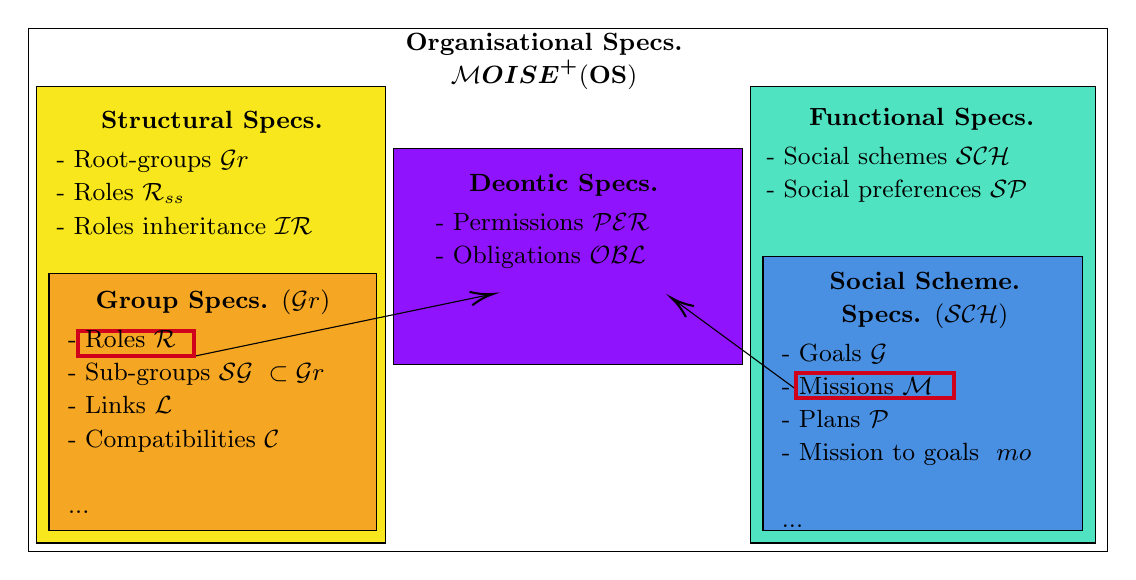
\begin{tikzpicture}[x=0.75pt,y=0.75pt,yscale=-1,xscale=1]
%uncomment if require: \path (0,1656); %set diagram left start at 0, and has height of 1656

%Shape: Rectangle [id:dp6756844921493015] 
\draw  [fill={rgb, 255:red, 248; green, 231; blue, 28 }  ,fill opacity=1 ] (46,1204) -- (214,1204) -- (214,1424) -- (46,1424) -- cycle ;
%Shape: Rectangle [id:dp3759944257810566] 
\draw  [fill={rgb, 255:red, 80; green, 227; blue, 194 }  ,fill opacity=1 ] (390,1204) -- (556,1204) -- (556,1424) -- (390,1424) -- cycle ;
%Shape: Rectangle [id:dp28244406216006945] 
\draw  [fill={rgb, 255:red, 144; green, 19; blue, 254 }  ,fill opacity=1 ] (218,1234) -- (386,1234) -- (386,1338) -- (218,1338) -- cycle ;
%Shape: Rectangle [id:dp32232123359581766] 
\draw   (42,1176) -- (562,1176) -- (562,1428) -- (42,1428) -- cycle ;
%Shape: Rectangle [id:dp7605706269262755] 
\draw  [fill={rgb, 255:red, 74; green, 144; blue, 226 }  ,fill opacity=1 ] (396,1286) -- (550,1286) -- (550,1418) -- (396,1418) -- cycle ;
%Shape: Rectangle [id:dp33110985390647496] 
\draw   (52,1294) -- (210,1294) -- (210,1418) -- (52,1418) -- cycle ;
%Shape: Rectangle [id:dp8653560038381976] 
\draw  [fill={rgb, 255:red, 245; green, 166; blue, 35 }  ,fill opacity=1 ] (52,1294) -- (210,1294) -- (210,1418) -- (52,1418) -- cycle ;
%Straight Lines [id:da09781093164567278] 
\draw    (412,1350) -- (353.61,1307.18) ;
\draw [shift={(352,1306)}, rotate = 36.25] [color={rgb, 255:red, 0; green, 0; blue, 0 }  ][line width=0.75]    (10.93,-3.29) .. controls (6.95,-1.4) and (3.31,-0.3) .. (0,0) .. controls (3.31,0.3) and (6.95,1.4) .. (10.93,3.29)   ;
%Straight Lines [id:da3938396723807833] 
\draw    (122,1334) -- (264.04,1304.41) ;
\draw [shift={(266,1304)}, rotate = 168.23] [color={rgb, 255:red, 0; green, 0; blue, 0 }  ][line width=0.75]    (10.93,-3.29) .. controls (6.95,-1.4) and (3.31,-0.3) .. (0,0) .. controls (3.31,0.3) and (6.95,1.4) .. (10.93,3.29)   ;
%Shape: Rectangle [id:dp269311335478327] 
\draw  [color={rgb, 255:red, 208; green, 2; blue, 27 }  ,draw opacity=1 ][line width=1.5]  (66,1322) -- (122,1322) -- (122,1334) -- (66,1334) -- cycle ;
%Shape: Rectangle [id:dp7449860119164387] 
\draw  [color={rgb, 255:red, 208; green, 2; blue, 27 }  ,draw opacity=1 ][line width=1.5]  (412,1342) -- (488,1342) -- (488,1354) -- (412,1354) -- cycle ;


% Text Node
\draw (472.5,1237.41) node   [align=left] {\begin{minipage}[lt]{112.2pt}\setlength\topsep{0pt}
\begin{center}
\textbf{{\small Functional Specs.}}
\end{center}
{\small  - Social schemes $\displaystyle \mathcal{SCH}$}\\{\small  - Social preferences $\displaystyle \mathcal{SP}$}
\end{minipage}};
% Text Node
\draw (474,1355) node   [align=left] {\begin{minipage}[lt]{103.36pt}\setlength\topsep{0pt}
\begin{center}
\textbf{{\small Social Scheme.}}\\{\small \textbf{Specs. }$\displaystyle (\mathcal{SCH})$}
\end{center}
{\small  - Goals $\displaystyle \mathcal{G}$}\\{\small  - Missions $\displaystyle \mathcal{M}$}\\{\small  - Plans $\displaystyle \mathcal{P}$}\\{\small  - Mission to goals \ $\displaystyle mo$}\\\\{\small  ...}
\end{minipage}};
% Text Node
\draw (131,1356) node   [align=left] {\begin{minipage}[lt]{104.72pt}\setlength\topsep{0pt}
\begin{center}
{\small \textbf{Group Specs. }$\displaystyle (\mathcal{G} r)$}
\end{center}
{\small  - Roles $\displaystyle \mathcal{R}$}\\{\small  - Sub-groups $\displaystyle \mathcal{SG} \ \subset \mathcal{G} r$}\\{\small  - Links $\displaystyle \mathcal{L}$}\\{\small  - Compatibilities $\displaystyle \mathcal{C}$}\\\\{\small  ...}
\end{minipage}};
% Text Node
\draw (181,1177) node [anchor=north west][inner sep=0.75pt]   [align=left] {\begin{minipage}[lt]{162.41pt}\setlength\topsep{0pt}
\begin{center}
{\small \textbf{Organisational Specs. }$\displaystyle \mathcal{M}\boldsymbol{OISE^{+}}$($\displaystyle \mathbf{OS}$)}
\end{center}

\end{minipage}};
% Text Node
\draw (300,1269.09) node   [align=left] {\begin{minipage}[lt]{92.48pt}\setlength\topsep{0pt}
\begin{center}
\textbf{{\small Deontic Specs.}}
\end{center}
{\small  - Permissions $\displaystyle \mathcal{PER}$}\\{\small  - Obligations $\displaystyle \mathcal{OBL}$}
\end{minipage}};
% Text Node
\draw (130.5,1245.69) node   [align=left] {\begin{minipage}[lt]{112.2pt}\setlength\topsep{0pt}
\begin{center}
\textbf{{\small Structural Specs.}}
\end{center}
{\small  - Root-groups $\displaystyle \mathcal{G} r$}\\{\small  - Roles $\displaystyle \mathcal{R}_{ss}$}\\{\small  - Roles inheritance $\displaystyle \mathcal{IR}$}
\end{minipage}};


\end{tikzpicture}
    \caption{Vue synthétique du modèle $\mathcal{M}OISE^+$}
    \label{fig:moise_model}
\end{figure}

Le modèle $\mathcal{M}OISE^+$~\cite{Hubner2007} fournit une description formelle avancée d'une organisation, notamment pour la description formelle des politiques des agents (via les plans). Il prend explicitement en compte les aspects sociaux entre agents, là où AGR se concentre sur l'intégration de normes orientées conception. De plus, il propose une vision suffisamment détaillée de l'organisation pour être comprise selon différents points de vue. Une représentation visuelle des éléments formels de ce modèle est donné en \autoref{fig:moise_model}
En nous basant sur le formalisme de $\mathcal{M}OISE^+$~\cite{Hubner2007}, nous ne détaillons ici que les éléments minimaux utilisés dans notre approche.

\

\noindent \textbf{Spécifications organisationnelles}~: \quad $\mathcal{OS} = \langle \mathcal{SS}, \mathcal{FS}, \mathcal{DS} \rangle$, l'ensemble des spécifications organisationnelles, où $\mathcal{SS}$ sont les \textbf{spécifications structurelles}, $\mathcal{FS}$ les \textbf{spécifications fonctionnelles}, et $\mathcal{DS}$ les \textbf{spécifications déontiques}.

\

\noindent \textbf{Spécifications Structurelles}~: \quad $\mathcal{SS} = \langle \mathcal{R}, \mathcal{IR}, \mathcal{G} \rangle$, où~:

\begin{itemize}
    \item $\mathcal{R}_{ss}$~: l'ensemble des rôles (notés $\rho \in \mathcal{R}$)~;
    \item $\mathcal{IR}: \mathcal{R} \rightarrow \mathcal{R}$~: la relation d'héritage entre rôles ($\mathcal{IR}(\rho_1) = \rho_2$ signifie que $\rho_1$ hérite de $\rho_2$, noté aussi $\rho_1 \sqsubset \rho_2$)~;
    \item $RG \subseteq GR$~: l'ensemble des groupes racines, $GR = \langle \mathcal{R}, \mathcal{SG}, \mathcal{L}^{intra}, \mathcal{L}^{inter}, \mathcal{C}^{intra}, \mathcal{C}^{inter}, np, ng \rangle$, l'ensemble des groupes, où~:
          \begin{itemize}
              \item $\mathcal{R} \subseteq \mathcal{R}_{ss}$~: l'ensemble des rôles non-abstraits~;
              \item $\mathcal{SG} \subseteq \mathcal{GR}$~: l'ensemble des sous-groupes~;
              \item $\mathcal{L} = \mathcal{R} \times \mathcal{R} \times \mathcal{TL}$~: l'ensemble des liens. Un lien est un triplet $(\rho_s,\rho_d,t) \in \mathcal{L}$ (aussi noté $link(\rho_s,\rho_d,t)$), où $\rho_s$ est le rôle source, $\rho_d$ le rôle destination, et $t \in \mathcal{TL}, \mathcal{TL} = \{acq, com, aut\}$ le type de lien~:
                    \begin{itemize}
                        \item $t = acq$ (acquaintance)~: les agents jouant $\rho_s$ peuvent identifier les agents jouant $\rho_d$~;
                        \item $t = com$ (communication)~: les agents jouant $\rho_s$ peuvent communiquer avec ceux jouant $\rho_d$~;
                        \item $t = aut$ (authority)~: les agents jouant $\rho_s$ peuvent exercer une autorité sur ceux jouant $\rho_d$. Ce lien nécessite les liens d'acquaintance et de communication.
                    \end{itemize}
              \item $\mathcal{L}^{intra} \subseteq \mathcal{L}$~: ensemble des liens intra-groupe~;
              \item $\mathcal{L}^{inter} \subseteq \mathcal{L}$~: ensemble des liens inter-groupe~;
              \item $\mathcal{C} = \mathcal{R} \times \mathcal{R}$~: l'ensemble des compatibilités. Une compatibilité est un couple $(\rho_a, \rho_b) \in \mathcal{C}$ (noté aussi $\rho_a \bowtie \rho_b$), signifiant qu'un agent jouant $\rho_a$ peut aussi jouer $\rho_b$~;
              \item $\mathcal{C}^{intra} \subseteq \mathcal{C}$~: ensemble des compatibilités intra-groupe~;
              \item $\mathcal{C}^{inter} \subseteq \mathcal{C}$~: ensemble des compatibilités inter-groupe~;
              \item $np: \mathcal{R} \rightarrow \mathbb{N} \times \mathbb{N}$~: relation donnant la cardinalité du nombre d'agents par rôle~;
              \item $ng: \mathcal{SG} \rightarrow \mathbb{N} \times \mathbb{N}$~: relation donnant la cardinalité de chaque sous-groupe.
          \end{itemize}
\end{itemize}

\medskip

\noindent \textbf{Spécifications Fonctionnelles}~: \quad $\mathcal{FS} = \langle \mathcal{SCH}, \mathcal{PO} \rangle$, où~:

\begin{itemize}
    \item $\mathcal{SCH} = \langle\mathcal{G}, \mathcal{M}, \mathcal{P}, mo, nm \rangle$~: l'ensemble des \textbf{schémas sociaux}, où~:
          \begin{itemize}
              \item $\mathcal{G}$~: l'ensemble des objectifs globaux~;
              \item $\mathcal{M}$~: l'ensemble des missions~;
              \item $\mathcal{P} = \langle \mathcal{G}, \{\mathcal{G}\}^s, OP, [0,1] \rangle, s \in \mathbb{N}^*$~: ensemble des plans qui définissent l'arbre des objectifs.
                    Un plan $p \in \mathcal{P}$ est un 4-uplet $p = (g_f, \{g_i\}_{0 \leq i \leq s}, op, p)$, où $g_f \in \mathcal{G}$ est un objectif, les $g_i \in \mathcal{G}$ sont des sous-objectifs, $op \in OP = \{sequence, choice, parallel\}$ est un opérateur, et $p \in [0,1]$ est une probabilité de succès~:
                    \begin{itemize}
                        \item $op = sequence$~: les $g_i$ doivent être atteints dans un ordre précis~;
                        \item $op = choice$~: un seul $g_i$ doit être atteint~;
                        \item $op = parallel$~: les $g_i$ peuvent être atteints en parallèle ou séquentiellement.
                    \end{itemize}
              \item $mo: \mathcal{M} \rightarrow \mathbb{P}(\mathcal{G})$~: relation liant une mission à un ensemble de objectifs~;
              \item $nm: \mathcal{M} \rightarrow \mathbb{N} \times \mathbb{N}$~: cardinalité du nombre d'agents affectés à une mission.
          \end{itemize}
    \item $\mathcal{PO}: \mathcal{M} \times \mathcal{M}$~: ensemble des \textbf{ordres de préférence}. Un ordre de préférence est un couple $(m_1, m_2)$ (noté aussi $m_1 \prec m_2$) signifiant que si un agent peut s'engager à la fois sur $m_1$ et $m_2$, il aura une préférence sociale pour $m_1$.
\end{itemize}

\medskip

\noindent \textbf{Spécifications Déontiques}~: \quad $\mathcal{DS} = \langle \mathcal{OBL}, \mathcal{PER} \rangle$, l'ensemble des spécifications déontiques, où~:

\begin{itemize}
    \item $\mathcal{TC}$~: ensemble des \textbf{contraintes temporelles}. Une contrainte $tc \in \mathcal{TC}$ indique les périodes pendant lesquelles une permission ou obligation est valide ($Any \in \mathcal{TC}$ signifie tout le temps)~;
    \item $\mathcal{OBL}: \mathcal{R} \times \mathcal{M} \times \mathcal{TC}$~: ensemble des \textbf{obligations}. Une obligation est un triplet $(\rho_a, m, tc)$ (aussi noté $obl(\rho_a, m, tc)$), signifiant qu'un agent jouant le rôle $\rho_a$ est obligé de s'engager dans la mission $m$ pendant la période spécifiée $tc$~;
    \item $\mathcal{PER}$~: ensemble des \textbf{permissions}. Une permission est un triplet $(\rho_a, m, tc)$ (aussi noté $per(\rho_a, m, tc)$), signifiant qu'un agent jouant le rôle $\rho_a$ est autorisé à s'engager dans la mission $m$ pendant $tc$.
\end{itemize}

\

\noindent Les spécifications organisationnelles appliquées aux agents sont les rôles et les objectifs (en tant que missions) à travers les permissions ou obligations. En effet, les autres spécifications structurelles comme les compatibilités ou les liens sont inhérentes aux rôles. De même, nous considérons que les objectifs, missions et leur association ($mo$) permettent de relier les autres spécifications fonctionnelles comme les plans, les cardinalités ou les préférences.
Par conséquent, nous considérons qu'il est suffisant de prendre en compte les rôles, les missions (objectifs et correspondance) et les permissions/obligations pour décrire l'essentiel de l'organisation d'un SMA.


\subsection{Liaison de \(\mathcal{M}OISE^+\) avec le MARL}

\begin{figure}[h!]

    \adjustbox{lap=-0.38cm}{\tikzset{every picture/.style={line width=0.75pt}} %set default line width to 0.75pt        

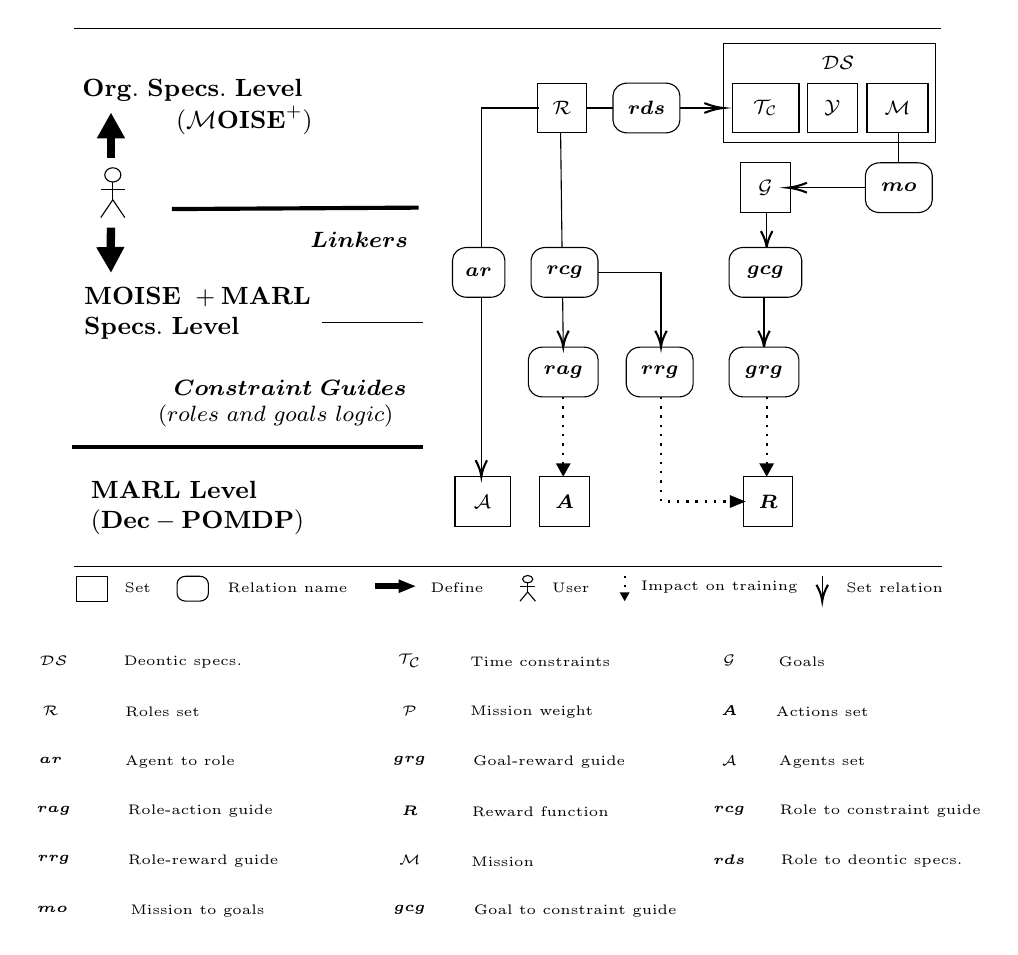
\begin{tikzpicture}[x=0.75pt,y=0.75pt,yscale=-1.2,xscale=1.4]
    %uncomment if require: \path (0,2584); %set diagram left start at 0, and has height of 2584

    %Straight Lines [id:da4973066741986565] 
    \draw [line width=1.5]    (118.21,2302.58) -- (203.1,2302) ;
    %Straight Lines [id:da14807114776731778] 
    \draw    (368.35,2272) -- (368.35,2294) -- (332.16,2294) ;
    \draw [shift={(330.16,2294)}, rotate = 360] [color={rgb, 255:red, 0; green, 0; blue, 0 }  ][line width=0.75]    (6.56,-1.97) .. controls (4.17,-0.84) and (1.99,-0.18) .. (0,0) .. controls (1.99,0.18) and (4.17,0.84) .. (6.56,1.97)   ;
    %Straight Lines [id:da16285043353898754] 
    \draw [line width=1.5]    (83.88,2398) -- (204.61,2398) ;
    %Straight Lines [id:da6299512000169913] 
    \draw    (169.94,2348) -- (204.61,2348) ;
    %Straight Lines [id:da64750232417664] 
    \draw    (84.65,2446) -- (383.15,2446) ;
    %Straight Lines [id:da35895220906699743] 
    \draw    (84.65,2230) -- (383,2230) ;
    %Straight Lines [id:da715014372569708] 
    \draw    (244.68,2262) -- (224.68,2262) -- (224.68,2408) ;
    \draw [shift={(224.68,2410)}, rotate = 270] [color={rgb, 255:red, 0; green, 0; blue, 0 }  ][line width=0.75]    (6.56,-1.97) .. controls (4.17,-0.84) and (1.99,-0.18) .. (0,0) .. controls (1.99,0.18) and (4.17,0.84) .. (6.56,1.97)   ;
    %Straight Lines [id:da71870438525014] 
    \draw    (251.96,2328) -- (286.51,2328) -- (286.51,2356) ;
    \draw [shift={(286.51,2358)}, rotate = 270] [color={rgb, 255:red, 0; green, 0; blue, 0 }  ][line width=0.75]    (6.56,-1.97) .. controls (4.17,-0.84) and (1.99,-0.18) .. (0,0) .. controls (1.99,0.18) and (4.17,0.84) .. (6.56,1.97)   ;
    %Straight Lines [id:da6006267784187092] 
    \draw [line width=0.75]  [dash pattern={on 0.84pt off 2.51pt}]  (252.87,2378) -- (252.87,2407) ;
    \draw [shift={(252.87,2410)}, rotate = 270] [fill={rgb, 255:red, 0; green, 0; blue, 0 }  ][line width=0.08]  [draw opacity=0] (5.36,-2.57) -- (0,0) -- (5.36,2.57) -- cycle    ;
    %Straight Lines [id:da8743336135156266] 
    \draw    (322.88,2304) -- (322.88,2316) ;
    \draw [shift={(322.88,2318)}, rotate = 270] [color={rgb, 255:red, 0; green, 0; blue, 0 }  ][line width=0.75]    (6.56,-1.97) .. controls (4.17,-0.84) and (1.99,-0.18) .. (0,0) .. controls (1.99,0.18) and (4.17,0.84) .. (6.56,1.97)   ;
    %Straight Lines [id:da14641229967966152] 
    \draw [line width=0.75]  [dash pattern={on 0.84pt off 2.51pt}]  (322.88,2378) -- (322.88,2407) ;
    \draw [shift={(322.88,2410)}, rotate = 270] [fill={rgb, 255:red, 0; green, 0; blue, 0 }  ][line width=0.08]  [draw opacity=0] (5.36,-2.57) -- (0,0) -- (5.36,2.57) -- cycle    ;
    %Straight Lines [id:da9260929933425808] 
    \draw [line width=0.75]  [dash pattern={on 0.84pt off 2.51pt}]  (286.51,2378) -- (286.51,2420) -- (312.61,2420) ;
    \draw [shift={(315.61,2420)}, rotate = 180] [fill={rgb, 255:red, 0; green, 0; blue, 0 }  ][line width=0.08]  [draw opacity=0] (5.36,-2.57) -- (0,0) -- (5.36,2.57) -- cycle    ;
    %Straight Lines [id:da3057006030233673] 
    \draw [line width=0.75]  [dash pattern={on 0.84pt off 2.51pt}]  (274,2449.7) -- (274,2457) ;
    \draw [shift={(274,2460)}, rotate = 270] [fill={rgb, 255:red, 0; green, 0; blue, 0 }  ][line width=0.08]  [draw opacity=0] (3.57,-1.72) -- (0,0) -- (3.57,1.72) -- cycle    ;
    %Straight Lines [id:da07288166228322246] 
    \draw    (342,2449.98) -- (342,2458) ;
    \draw [shift={(342,2460)}, rotate = 270] [color={rgb, 255:red, 0; green, 0; blue, 0 }  ][line width=0.75]    (6.56,-1.97) .. controls (4.17,-0.84) and (1.99,-0.18) .. (0,0) .. controls (1.99,0.18) and (4.17,0.84) .. (6.56,1.97)   ;
    %Shape: Ellipse [id:dp8508274348425935] 
    \draw   (95.09,2288.86) .. controls (95.09,2287.28) and (96.33,2286) .. (97.85,2286) .. controls (99.38,2286) and (100.62,2287.28) .. (100.62,2288.86) .. controls (100.62,2290.44) and (99.38,2291.71) .. (97.85,2291.71) .. controls (96.33,2291.71) and (95.09,2290.44) .. (95.09,2288.86) -- cycle ;
    %Straight Lines [id:da3825450168053828] 
    \draw    (97.85,2291.71) -- (97.85,2298.86) ;
    %Straight Lines [id:da521321206042058] 
    \draw    (97.85,2298.86) -- (93.71,2306) ;
    %Straight Lines [id:da055514206493922025] 
    \draw    (97.85,2298.86) -- (102,2306) ;
    %Straight Lines [id:da8996496708356774] 
    \draw    (102,2294.57) -- (93.71,2294.57) ;

    %Straight Lines [id:da31678488015771755] 
    \draw [line width=2.25]    (188,2454) -- (196.97,2454) ;
    \draw [shift={(201.97,2454)}, rotate = 180] [fill={rgb, 255:red, 0; green, 0; blue, 0 }  ][line width=0.08]  [draw opacity=0] (5.72,-2.75) -- (0,0) -- (5.72,2.75) -- cycle    ;
    %Shape: Ellipse [id:dp3927356466672782] 
    \draw   (238.88,2451.17) .. controls (238.88,2450.36) and (239.67,2449.7) .. (240.64,2449.7) .. controls (241.61,2449.7) and (242.4,2450.36) .. (242.4,2451.17) .. controls (242.4,2451.99) and (241.61,2452.65) .. (240.64,2452.65) .. controls (239.67,2452.65) and (238.88,2451.99) .. (238.88,2451.17) -- cycle ;
    %Straight Lines [id:da3365602555559104] 
    \draw    (240.64,2452.65) -- (240.64,2456.32) ;
    %Straight Lines [id:da7990875235744026] 
    \draw    (240.64,2456.32) -- (238,2460) ;
    %Straight Lines [id:da23945649338821617] 
    \draw    (240.64,2456.32) -- (243.28,2460) ;
    %Straight Lines [id:da11927353559661591] 
    \draw    (243.28,2454.12) -- (238,2454.12) ;

    %Straight Lines [id:da5816423191130675] 
    \draw    (251.96,2272) -- (252.85,2356) ;
    \draw [shift={(252.87,2358)}, rotate = 269.39] [color={rgb, 255:red, 0; green, 0; blue, 0 }  ][line width=0.75]    (6.56,-1.97) .. controls (4.17,-0.84) and (1.99,-0.18) .. (0,0) .. controls (1.99,0.18) and (4.17,0.84) .. (6.56,1.97)   ;
    %Straight Lines [id:da9310455126832857] 
    \draw    (321.97,2338) -- (321.97,2356) ;
    \draw [shift={(321.97,2358)}, rotate = 270] [color={rgb, 255:red, 0; green, 0; blue, 0 }  ][line width=0.75]    (6.56,-1.97) .. controls (4.17,-0.84) and (1.99,-0.18) .. (0,0) .. controls (1.99,0.18) and (4.17,0.84) .. (6.56,1.97)   ;
    %Shape: Rectangle [id:dp293492578719597] 
    \draw   (120,2453) .. controls (120,2451.34) and (121.34,2450) .. (123,2450) -- (127.72,2450) .. controls (129.37,2450) and (130.72,2451.34) .. (130.72,2453) -- (130.72,2457) .. controls (130.72,2458.66) and (129.37,2460) .. (127.72,2460) -- (123,2460) .. controls (121.34,2460) and (120,2458.66) .. (120,2457) -- cycle ;
    %Straight Lines [id:da33566712615128225] 
    \draw    (261.05,2262) -- (306,2262) ;
    \draw [shift={(308,2262)}, rotate = 180] [color={rgb, 255:red, 0; green, 0; blue, 0 }  ][line width=0.75]    (6.56,-1.97) .. controls (4.17,-0.84) and (1.99,-0.18) .. (0,0) .. controls (1.99,0.18) and (4.17,0.84) .. (6.56,1.97)   ;
    %Shape: Rectangle [id:dp28383270948937667] 
    \draw   (308,2236) -- (381.08,2236) -- (381.08,2276) -- (308,2276) -- cycle ;
    %Straight Lines [id:da18020989903965012] 
    \draw [line width=3]    (97.22,2282) -- (97.22,2270) ;
    \draw [shift={(97.22,2264)}, rotate = 90] [fill={rgb, 255:red, 0; green, 0; blue, 0 }  ][line width=0.08]  [draw opacity=0] (10.18,-4.89) -- (0,0) -- (10.18,4.89) -- cycle    ;
    %Straight Lines [id:da018421338049046554] 
    \draw [line width=3]    (97.22,2310) -- (97.11,2322.37) ;
    \draw [shift={(97.22,2328)}, rotate = 268.86] [fill={rgb, 255:red, 0; green, 0; blue, 0 }  ][line width=0.08]  [draw opacity=0] (10.18,-4.89) -- (0,0) -- (10.18,4.89) -- cycle    ;
    %Shape: Rectangle [id:dp7281037051878541] 
    \draw   (85.42,2450) -- (96.13,2450) -- (96.13,2460) -- (85.42,2460) -- cycle ;

    % Text Node
    \draw (362,2544.5) node  [font=\tiny] [align=left] {Role to constraint guide};
    % Text Node
    \draw (342,2524.5) node  [font=\tiny] [align=left] {Agents set};
    % Text Node
    \draw (342,2504.5) node  [font=\tiny] [align=left] {Actions set};
    % Text Node
    \draw (257,2584.5) node  [font=\tiny] [align=left] {Goal to constraint guide};
    % Text Node
    \draw (335,2484.5) node  [font=\tiny] [align=left] {Goals};
    % Text Node
    \draw (359,2564.5) node  [font=\tiny] [align=left] {Role to deontic specs.};
    % Text Node
    \draw (232,2564.5) node  [font=\tiny] [align=left] {Mission};
    % Text Node
    \draw (245,2544.5) node  [font=\tiny] [align=left] {Reward function};
    % Text Node
    \draw (248,2524.5) node  [font=\tiny] [align=left] {Goal-reward guide};
    % Text Node
    \draw (242,2504.5) node  [font=\tiny] [align=left] {Mission weight};
    % Text Node
    \draw (245,2484.5) node  [font=\tiny] [align=left] {Time constraints};
    % Text Node
    \draw (127,2584.5) node  [font=\tiny] [align=left] {Mission to goals};
    % Text Node
    \draw (129,2564.5) node  [font=\tiny] [align=left] {Role-reward guide};
    % Text Node
    \draw (128,2544.5) node  [font=\tiny] [align=left] {Role-action guide};
    % Text Node
    \draw (121,2524.5) node  [font=\tiny] [align=left] {Agent to role};
    % Text Node
    \draw (115,2504.5) node  [font=\tiny] [align=left] {Roles set};
    % Text Node
    \draw (122,2484.5) node  [font=\tiny] [align=left] {Deontic specs.};
    % Text Node
    \draw (310,2544) node  [font=\tiny] [align=left] {$\displaystyle \boldsymbol{rcg}$};
    % Text Node
    \draw (200,2504) node  [font=\tiny] [align=left] {$\displaystyle \mathcal{P}$};
    % Text Node
    \draw (200,2484) node  [font=\tiny] [align=left] {$\displaystyle \mathcal{T_{C}}$};
    % Text Node
    \draw (200,2564) node  [font=\tiny] [align=left] {$\displaystyle \mathcal{M}$};
    % Text Node
    \draw (77.5,2484) node  [font=\tiny] [align=left] {$\displaystyle \mathcal{DS}$};
    % Text Node
    \draw (310,2564) node  [font=\tiny] [align=left] {$\displaystyle \boldsymbol{rds}$};
    % Text Node
    \draw (310,2504) node  [font=\tiny] [align=left] {$\displaystyle \boldsymbol{A}$};
    % Text Node
    \draw (200,2544) node  [font=\tiny] [align=left] {$\displaystyle \boldsymbol{R}$};
    % Text Node
    \draw (310,2524) node  [font=\tiny] [align=left] {$\displaystyle \mathcal{A}$};
    % Text Node
    \draw (200,2524) node  [font=\tiny] [align=left] {$\displaystyle \boldsymbol{grg}$};
    % Text Node
    \draw (77.5,2564) node  [font=\tiny] [align=left] {$\displaystyle \boldsymbol{rrg}$};
    % Text Node
    \draw (77.5,2544) node  [font=\tiny] [align=left] {$\displaystyle \boldsymbol{rag}$};
    % Text Node
    \draw (200,2584) node  [font=\tiny] [align=left] {$\displaystyle \boldsymbol{gcg}$};
    % Text Node
    \draw (76.5,2524) node  [font=\tiny] [align=left] {$\displaystyle \boldsymbol{ar}$};
    % Text Node
    \draw (77,2584) node  [font=\tiny] [align=left] {$\displaystyle \boldsymbol{mo}$};
    % Text Node
    \draw (76.5,2504) node  [font=\tiny] [align=left] {$\displaystyle \mathcal{R}$};
    % Text Node
    \draw (310,2484) node  [font=\tiny] [align=left] {$\displaystyle \mathcal{G}$};


    % Text Node
    \draw  [fill={rgb, 255:red, 255; green, 255; blue, 255 }  ,fill opacity=1 ]  (241.82,2323) .. controls (241.82,2320.24) and (244.06,2318) .. (246.82,2318) -- (259.82,2318) .. controls (262.58,2318) and (264.82,2320.24) .. (264.82,2323) -- (264.82,2333) .. controls (264.82,2335.76) and (262.58,2338) .. (259.82,2338) -- (246.82,2338) .. controls (244.06,2338) and (241.82,2335.76) .. (241.82,2333) -- cycle  ;
    \draw (253.32,2328) node  [font=\scriptsize] [align=left] {$\displaystyle \boldsymbol{rcg}$};
    % Text Node
    \draw    (337,2252) -- (354,2252) -- (354,2272) -- (337,2272) -- cycle  ;
    \draw (345.5,2262) node  [font=\scriptsize] [align=left] {$\displaystyle \mathcal{Y}$};
    % Text Node
    \draw    (311,2252) -- (334,2252) -- (334,2272) -- (311,2272) -- cycle  ;
    \draw (322.5,2262) node  [font=\scriptsize] [align=left] {$\displaystyle \mathcal{T_{C}}$};
    % Text Node
    \draw    (357.39,2252) -- (378.39,2252) -- (378.39,2272) -- (357.39,2272) -- cycle  ;
    \draw (367.89,2262) node  [font=\scriptsize] [align=left] {$\displaystyle \mathcal{M}$};
    % Text Node
    \draw (347.43,2244) node  [font=\scriptsize] [align=left] {$\displaystyle \mathcal{DS}$};
    % Text Node
    \draw  [fill={rgb, 255:red, 255; green, 255; blue, 255 }  ,fill opacity=1 ]  (270,2257) .. controls (270,2254.24) and (272.24,2252) .. (275,2252) -- (288,2252) .. controls (290.76,2252) and (293,2254.24) .. (293,2257) -- (293,2267) .. controls (293,2269.76) and (290.76,2272) .. (288,2272) -- (275,2272) .. controls (272.24,2272) and (270,2269.76) .. (270,2267) -- cycle  ;
    \draw (281.5,2262) node  [font=\scriptsize] [align=left] {$\displaystyle \boldsymbol{rds}$};
    % Text Node
    \draw (158,2454.5) node  [font=\tiny] [align=left] {Relation name};
    % Text Node
    \draw (106.46,2454.5) node  [font=\tiny] [align=left] {Set};
    % Text Node
    \draw (255.47,2454.5) node  [font=\tiny] [align=left] {User};
    % Text Node
    \draw (216.32,2454.5) node  [font=\tiny] [align=left] {Define};
    % Text Node
    \draw (366.91,2454.5) node  [font=\tiny] [align=left] {Set relation};
    % Text Node
    \draw (306.61,2454.5) node  [font=\tiny] [align=left] {Impact on training};
    % Text Node
    \draw    (244.82,2410) -- (261.82,2410) -- (261.82,2430) -- (244.82,2430) -- cycle  ;
    \draw (253.32,2420) node  [font=\scriptsize] [align=left] {$\displaystyle \boldsymbol{A}$};
    % Text Node
    \draw    (314.84,2410) -- (331.84,2410) -- (331.84,2430) -- (314.84,2430) -- cycle  ;
    \draw (323.34,2420) node  [font=\scriptsize] [align=left] {$\displaystyle \boldsymbol{R}$};
    % Text Node
    \draw    (215.63,2410) -- (234.63,2410) -- (234.63,2430) -- (215.63,2430) -- cycle  ;
    \draw (225.13,2420) node  [font=\scriptsize] [align=left] {$\displaystyle \mathcal{A}$};
    % Text Node
    \draw  [fill={rgb, 255:red, 255; green, 255; blue, 255 }  ,fill opacity=1 ]  (309.97,2363) .. controls (309.97,2360.24) and (312.21,2358) .. (314.97,2358) -- (328.97,2358) .. controls (331.73,2358) and (333.97,2360.24) .. (333.97,2363) -- (333.97,2373) .. controls (333.97,2375.76) and (331.73,2378) .. (328.97,2378) -- (314.97,2378) .. controls (312.21,2378) and (309.97,2375.76) .. (309.97,2373) -- cycle  ;
    \draw (321.97,2368) node  [font=\scriptsize] [align=left] {$\displaystyle \boldsymbol{grg}$};
    % Text Node
    \draw    (274.56,2363) .. controls (274.56,2360.24) and (276.8,2358) .. (279.56,2358) -- (292.56,2358) .. controls (295.32,2358) and (297.56,2360.24) .. (297.56,2363) -- (297.56,2373) .. controls (297.56,2375.76) and (295.32,2378) .. (292.56,2378) -- (279.56,2378) .. controls (276.8,2378) and (274.56,2375.76) .. (274.56,2373) -- cycle  ;
    \draw (286.06,2368) node  [font=\scriptsize] [align=left] {$\displaystyle \boldsymbol{rrg}$};
    % Text Node
    \draw    (240.87,2363) .. controls (240.87,2360.24) and (243.11,2358) .. (245.87,2358) -- (259.87,2358) .. controls (262.63,2358) and (264.87,2360.24) .. (264.87,2363) -- (264.87,2373) .. controls (264.87,2375.76) and (262.63,2378) .. (259.87,2378) -- (245.87,2378) .. controls (243.11,2378) and (240.87,2375.76) .. (240.87,2373) -- cycle  ;
    \draw (252.87,2368) node  [font=\scriptsize] [align=left] {$\displaystyle \boldsymbol{rag}$};
    % Text Node
    \draw (156.15,2380.5) node  [font=\footnotesize] [align=left] {$\displaystyle  \begin{array}{{>{\displaystyle}l}}
                \ \ \boldsymbol{Constraint\ Guides} \\
                ( roles\ and\ goals\ logic)
            \end{array}$};
    % Text Node
    \draw  [fill={rgb, 255:red, 255; green, 255; blue, 255 }  ,fill opacity=1 ]  (309.93,2323) .. controls (309.93,2320.24) and (312.17,2318) .. (314.93,2318) -- (329.93,2318) .. controls (332.69,2318) and (334.93,2320.24) .. (334.93,2323) -- (334.93,2333) .. controls (334.93,2335.76) and (332.69,2338) .. (329.93,2338) -- (314.93,2338) .. controls (312.17,2338) and (309.93,2335.76) .. (309.93,2333) -- cycle  ;
    \draw (322.43,2328) node  [font=\scriptsize] [align=left] {$\displaystyle \boldsymbol{gcg}$};
    % Text Node
    \draw  [fill={rgb, 255:red, 255; green, 255; blue, 255 }  ,fill opacity=1 ]  (214.77,2323) .. controls (214.77,2320.24) and (217.01,2318) .. (219.77,2318) -- (227.77,2318) .. controls (230.53,2318) and (232.77,2320.24) .. (232.77,2323) -- (232.77,2333) .. controls (232.77,2335.76) and (230.53,2338) .. (227.77,2338) -- (219.77,2338) .. controls (217.01,2338) and (214.77,2335.76) .. (214.77,2333) -- cycle  ;
    \draw (223.77,2328) node  [font=\scriptsize] [align=left] {$\displaystyle \boldsymbol{ar}$};
    % Text Node
    \draw  [fill={rgb, 255:red, 255; green, 255; blue, 255 }  ,fill opacity=1 ]  (356.85,2289) .. controls (356.85,2286.24) and (359.08,2284) .. (361.85,2284) -- (374.85,2284) .. controls (377.61,2284) and (379.85,2286.24) .. (379.85,2289) -- (379.85,2299) .. controls (379.85,2301.76) and (377.61,2304) .. (374.85,2304) -- (361.85,2304) .. controls (359.08,2304) and (356.85,2301.76) .. (356.85,2299) -- cycle  ;
    \draw (368.35,2294) node  [font=\scriptsize] [align=left] {$\displaystyle \boldsymbol{mo}$};
    % Text Node
    \draw (127,2344.5) node  [font=\small] [align=left] {$\displaystyle  \begin{array}{{>{\displaystyle}l}}
                \mathbf{MOISE\ +MARL} \\
                \mathbf{Specs.\ Level}
            \end{array}$};
    % Text Node
    \draw (127,2422.5) node  [font=\small] [align=left] {$\displaystyle  \begin{array}{{>{\displaystyle}l}}
                \mathbf{MARL\ Level} \\
                \mathbf{(Dec-POMDP)}
            \end{array}$};
    % Text Node
    \draw    (243.91,2252) -- (260.91,2252) -- (260.91,2272) -- (243.91,2272) -- cycle  ;
    \draw (252.41,2262) node  [font=\scriptsize] [align=left] {$\displaystyle \mathcal{R}$};
    % Text Node
    \draw (182.64,2315) node  [font=\footnotesize] [align=left] {$\displaystyle \boldsymbol{Linkers}$};
    % Text Node
    \draw    (313.93,2284) -- (330.93,2284) -- (330.93,2304) -- (313.93,2304) -- cycle  ;
    \draw (322.43,2294) node  [font=\scriptsize] [align=left] {$\displaystyle \mathcal{G}$};
    % Text Node
    \draw (127,2261.5) node  [font=\small] [align=left] {$\displaystyle  \begin{array}{{>{\displaystyle}l}}
                \mathbf{{\displaystyle Org.\ Specs.\ Level}} \\
                {\displaystyle \ \ \ \ \ \ \ \ \ \ \ (\mathcal{M}\mathbf{OISE^+})}
            \end{array}$};


\end{tikzpicture}}
    \caption{\textbf{Une vue minimale du cadre MOISE+MARL} :
        Les utilisateurs définissent d'abord les spécifications de \(\mathcal{M}OISE^+\), qui incluent des rôles (\(\mathcal{R}\)) et des missions (\(\mathcal{M}\)) associées via \(rds\). Ensuite, ils créent des spécifications MOISE+MARL en définissant d'abord des \textbf{Guides de Contraintes} tels que \(rag\) et \(rrg\) pour spécifier la logique des rôles, et \(grg\) pour la logique des objectifs.
        Ensuite, des \textbf{Lieurs} sont utilisés pour connecter les agents aux rôles via \(ar\) et pour relier la logique des \textbf{Guides de Contrainte} aux spécifications définies de \(\mathcal{M}OISE^+\). Une fois cette configuration réalisée, des rôles peuvent être attribués aux agents, et le cadre MARL s'adapte en conséquence pendant l'entraînement.
    }
    \label{fig:mm_synthesis}
\end{figure}

Alors qu'\textit{AGR}~\cite{ferber2003} est un cadre informel qui introduit des rôles par groupes, \(\mathcal{M}OISE^+\) offre une description plus détaillée et flexible des structures et fonctions d'un système multi-agent (MAS), facilitant ainsi la formalisation des politiques en MARL.

\medskip
\noindent \textbf{Guides de Contraintes} : Trois relations décrivent la logique des rôles et objectifs dans le cadre Dec-POMDP :

\begin{itemize}
    \item \textbf{Guide d'action de rôle} \(rag: H \times \Omega \to \mathcal{P}(A \times \mathbb{R})\) : Pour chaque couple \((h,\omega)\) (\(h\in H\), \(\omega\in \Omega\)), il associe un ensemble d'actions \(A_\omega \subseteq A\) avec une rigidité \(ch \in [0,1]\) (par défaut \(ch=1\)), restreignant ainsi le choix de la prochaine action ;
    \item \textbf{Guide de récompense de rôle} \(rrg: H \times \Omega \times A \to \mathbb{R}\) : Défini par \(rrg(h,\omega,a)=r_m\) si \(a \notin A_\omega\) (avec \(rag(h,\omega)=A_\omega \times \mathbb{R}\)), et 0 sinon, afin d'encourager le respect du rôle ;
    \item \textbf{Guide de récompense d'objectif} \(grg: H \to \mathbb{R}\) : Attribue un bonus \(r_b\) à la récompense globale si \(h\) contient une sous-séquence caractéristique \(h_g \in H_g\) correspondant à un objectif.
\end{itemize}


\medskip
\noindent \textbf{Lieurs} : Relient les spécifications de \(\mathcal{M}OISE^+\) aux Guides de Contraintes et aux agents :

\begin{itemize}
    \item \textbf{Agent vers Rôle} \(ar: \mathcal{A} \to \mathcal{R}\) (relation bijective) ;
    \item \textbf{Rôle vers Guide de Contrainte} \(rcg: \mathcal{R} \to rag \cup rrg\) : Associe à chaque rôle une relation \(rag\) ou \(rrg\) ;
    \item \textbf{Objectif vers Guide de Contrainte} \(gcg: \mathcal{G} \to grg\) : Relie chaque objectif à son guide \(grg\).
\end{itemize}

\begin{figure*}[h!]
    \label{eq:single_value_function}
    \raggedright
    \textbf{\textit{Definition 1} \quad Fonction État-Valeur adaptée aux guides de contraintes en AEC :}

    \begin{scriptsize}
        \vspace{0.cm}
        \begin{gather*}
            V^{\pi^j}(s_t) = \hspace{-0.75cm}
            %
            \sum_{\textcolor{red}{ \substack{a_{t} \in A \text{ if } rn() < ch_{t}, \\
                        a_{t} \in A_{t} \text{ else}}
                }}{\hspace{-0.7cm} \pi_i(a_{t} | \omega_t)}
            %
            \sum_{s_{t+1} \in S}
            %
            {\hspace{-0.1cm} T(s_{t+1} | s_t, a_{t})
            \Bigl[R(s_t,a_{t},s_{t+1}) + \hspace{-0.1cm}
            \textcolor{blue}{ \sum_{m \in \mathcal{M}_i}{ \hspace{-0.1cm} v_m(t) \frac{grg_m(h_{t+1})}{1 - p + \epsilon} } }
            + } \\
            {\hspace{6cm}\textcolor{red}{(1-ch_t) \times rrg(\omega_t,a_{t+1})} + V^{\pi^j_{i+1 \ mod \ n}}(s_{t+1})\Bigr]}
        \end{gather*}
        %
        \vspace{0.cm}
        \textcolor{red}{\[\text{ \hspace{-0.3cm} Avec } rag(h_t, \omega_t) = A_{t} \times \mathbb{R} \text{, } \langle a_t, ch_{t} \rangle \in A_{t} \times \mathbb{R} \text{ ; } rn: \emptyset \to [0,1[ \text{, une fonction aléatoire uniforme}\]}
        %
        \vspace{-0.2cm}
        \textcolor{blue}{
            \begin{gather*}
                \hspace{-0.65cm}
                \text{Avec } \omega_t = O(\omega_t | s_t, a_t) \text{ ; } h_t = \{h_0 = \langle \rangle, h_{t+1} = \langle h_t, \langle \omega_{t+1}, a_{t+1} \rangle \rangle \} \text{ ; } \epsilon \in \mathbb{R}_{>0} \text{ ; } grg_m(h) =
            \end{gather*}
        }
        \vspace{-0.2cm}
        \textcolor{blue}{
            \begin{gather*}
                \hspace{-0.5cm} \sum_{\hspace{0.3cm}(grg_i,w_i) \in mo(m)}{\hspace{-0.9cm} w_i \times grg_i(h)}
                \text{ ; } v_m(t) = \{ 1 \text{ if } t \in t_c \text{ ; else } 0 \} \text{ ; } \mathcal{M}_i = \{m_j | \langle ar(i),m_j,t_c,p \rangle \in \mathcal{M}\}
            \end{gather*}
        }
        \vspace{0.cm}
    \end{scriptsize}

\end{figure*}


\textbf{La résolution du problème MOISE+MARL} consiste à trouver une politique conjointe
$
    \pi^j = \{\pi^j_0, \pi^j_1, \dots, \pi^j_n\}
$
maximisant la fonction de valeur d'état \(V^{\pi^j}\) (ou atteignant un seuil minimal), qui représente la récompense cumulative attendue à partir d'un état initial \(s \in S\) en suivant les actions conjointes \(a^j \in A^n\) sous l'effet de \textbf{Guides de Contraintes}. Cette fonction est définie pour des agents agissant de manière séquentielle et cyclique (mode \textit{Agent Environment Cycle} -- AEC) (voir la \hyperref[eq:single_value_function]{Définition 1}). La \autoref{fig:mm_synthesis} illustre les liens entre \(\mathcal{M}OISE^+\) et le Dec-POMDP via MOISE+MARL.

À chaque instant \(t \in \mathbb{N}\) (initialement \(t=0\)), l'agent \(i = t \mod n\) doit assumer le rôle \(\rho_i = ar(i)\). Pour chaque spécification déontique valide
$
    d_i = rds(\rho_i) = \langle tc_i, y_i, m_i \rangle,
$
l'agent est autorisé (si \(y_i=0\)) ou obligé (si \(y_i=1\)) d'exécuter la mission \(m_i \in \mathcal{M}\) (avec \(\mathcal{G}_{m_i} = mo(m_i)\)). L'agent choisit d'abord une action parmi celles attendues \(A_t\) si une valeur aléatoire est inférieure à la rigidité \(ch_t\), sinon parmi l'ensemble \(A\); ainsi, un \(ch_t = 1\) impose une contrainte forte.

L'action appliquée à \(s_t\) conduit à l'état suivant \(s_{t+1}\), génère la prochaine observation \(\omega_{t+1}\) et une récompense. Celle-ci est la somme de la récompense globale et des ajustements organisationnels :
i) un bonus (via les Guides de Récompense d'Objectif), pondéré par \(\frac{1}{1-p+\epsilon}\) pour ajuster son impact, et
ii) une pénalité (via les Guides de Récompense de Rôle), pondérée par la rigidité \(ch_t\) pour ajuster son impact.
Le calcul de la récompense cumulative se poursuit dans \(s_{t+1}\) avec l'agent suivant \((i+1) \mod n\).

\subsection{Faciliter l'implémentation des \textbf{Guides de Contrainte}}

Puisque les rôles, objectifs et missions sont de simples étiquettes, leur définition est implicite. Cependant, implémenter une relation \(rag\), \(rrg\) ou \(grg\) nécessite de définir de nombreux historiques, souvent redondants, rendant une définition extensionnelle fastidieuse et peu évolutive. De plus, la logique de chaque \textbf{Guide de Contrainte} repose sur l’analyse de trajectoires d’agents : pour chaque historique observé, il faut décider s’il appartient à un ensemble d’historiques attendus et quelles conséquences en tirer (masquage d’actions, ajout de pénalités ou de bonus de récompense). Par exemple, \(rag\) restreint les actions disponibles selon l’appartenance de la trajectoire courante à un ensemble \(H_g\) et la nouvelle observation.

Une première approche consiste à laisser l’utilisateur définir ces guides par une logique procédurale (scripts Python ou règles spécifiques). Dans ce cas, la relation \(b_g: H \to \{0,1\}\) formalise la décision d’appartenance d’un historique à un ensemble \(H_g\). Cette solution est flexible, car elle peut exploiter la totalité du contexte disponible (positions spatiales, états internes, séquences passées). Toutefois, elle reste coûteuse à écrire et à maintenir, et conduit souvent à des définitions très verbeuses.

Pour dépasser cette limite, nous introduisons les \textit{Trajectory-based Patterns} (TPs), inspirés du Traitement Automatique du Langage. L’idée est de fournir un formalisme déclaratif compact permettant d’exprimer des comportements attendus comme des motifs temporels. Un TP \(p \in P\) correspond ainsi à un patron qui capture un ensemble d’historiques de manière intentionnelle. Chaque observation ou action est associée à une étiquette \(l \in L\) (via \(l: \Omega \cup A \to L\)), ce qui rend la manipulation pratique et indépendante des détails bas-niveau de l’environnement.
%
Un TP \(p\) peut être :
\begin{itemize}
    \item une \textbf{séquence feuille} \(s_l = \langle h, \{c_{min}, c_{max}\} \rangle\), où \(h \in H\) désigne une sous-séquence observation/action et \(\{c_{min}, c_{max}\}\) est la cardinalité ;
    \item une \textbf{séquence nœud} \(s_n = \langle \langle s_{l_1}, s_{l_2}, \dots \rangle, \{c_{min}, c_{max}\} \rangle\), combinant plusieurs séquences en un motif hiérarchique.
\end{itemize}

\noindent
Par exemple, le pattern
%
$p = ``[o_1,a_1,[o_2,a_2]\langle0,2\rangle]\langle1,*\rangle"$
%
se lit comme suit : un historique valide doit contenir au moins une occurrence de la paire \(\langle o_1,a_1\rangle\), suivie de zéro à deux occurrences de \(\langle o_2,a_2\rangle\). Ce TP capture donc une famille entière de comportements, sans avoir à lister tous les historiquess.
%
% La relation de correspondance est alors définie par :
% \[
%     b_g(h) = m(p_g,h), \quad \text{avec } m: P \times H \to \{0,1\},
% \]
% où \(m(p_g,h)\) indique si un historique \(h \in H\) satisfait le pattern \(p_g \in P\).
%
L’intérêt des TPs est double :
\begin{enumerate*}[label={\roman*) },itemjoin={; \quad}]
    \item Ils permettent de coder de manière \textbf{compacte} des comportements étendus dans le temps, difficiles à exprimer autrement.
    \item Ils facilitent la \textbf{réutilisation}, puisque les mêmes motifs peuvent être partagés entre plusieurs rôles ou objectifs.
\end{enumerate*}

\paragraph{Exemple concret.} Considérons l’environnement \textit{Overcooked-AI}, où des agents cuisiniers doivent collaborer en se déplaçant dans un monde en grille et interagir avec les ingrédient (oignons) et les instruments (pots, bols) pour faire de la soupe qui est expédiée en interagissant avec la zone d'expedition. Ici, l’on souhaite reconnaître le comportement suivant : \textquote{un agent qui détient un oignon, observe un pot et interagit avec lui pour le remplir}. Ce comportement peut être exprimé par le TP suivant :
\[
    p = [[\#any](*) , \; has\_onion , \; [\#any](*) , \; see\_pot , \; interact \;](1,1)
\]

\noindent
Ce TP peut être exploité dans les guides de contrainte comme montré dans la \autoref{tab:tp_guides_example} pour inciter l'agent à intéragir à nouveau pour récupérer la soupe par exemple.

\begin{table}[h]
    \centering
    \caption{Exemple de guides appliqués au TP ``remplir un pot avec un oignon''.}
    \label{tab:tp_guides_example}
    \scriptsize
    \renewcommand{\arraystretch}{1.3}
    % \setlength{\tabcolsep}{10pt}
    \begin{tabular}{p{2cm}@{\hspace{20pt}}p{6cm}}
        \hline
        \textbf{Guide}                            & \textbf{Exemple de règle}                                         \\
        \hline
        \textbf{RAG} (\textit{Role Action Guide}) & Si le TP est satisfait, restreindre les actions possibles~:
        \[
            rag(h,\omega) = \{\texttt{interact} \mapsto 1.0, \;\texttt{nothing} \mapsto 0.2\}
        \]
        L’action \texttt{interact} est fortement favorisée.                                                           \\
        \hdashline
        \textbf{RRG} (\textit{Role Reward Guide}) & Ajouter un bonus de rôle lorsque l’action attendue est réalisée~:
        \[
            rrg(h,\omega,a) =
            \begin{cases}
                +3 & \text{si } a = \texttt{interact} \\
                0  & \text{sinon}
            \end{cases}
        \]                                                                                                            \\
        \hdashline
        \textbf{GRG} (\textit{Goal Reward Guide}) & Accorder une récompense si le TP est détecté / atteint~:
        \[
            grg(h) =
            \begin{cases}
                +5 & \text{si le pot est rempli (TP reconnu)} \\
                0  & \text{sinon}
            \end{cases}
        \]                                                                                                            \\
        \hline
    \end{tabular}
\end{table}

Ainsi, au lieu de définir extensionnellement de vastes ensembles \(H_g\), l’utilisateur décrit quelques motifs symboliques qui capturent l’essence des comportements recherchés. MOISE+MARL applique alors automatiquement ces motifs aux guides (\(rag, rrg, grg\)), rendant leur mise en œuvre plus modulaire, scalable et interprétable.


\section{La méthode TEMM}
\label{sec:TEMM_algorithm}

Comme indiqué en \autoref{sec:related_works}, aucun travaux ne répond pleinement à nos exigences pour déterminer les rôles et objectifs implicites ainsi que l'adéquation organisationnelle. Nous proposons donc la méthode TEMM, qui vise à extraire automatiquement des spécifications organisationnelles \(\mathcal{M}OISE^+\) implicites à partir des trajectoires d’agents entraînés.

On suppose qu'une politique d'agent donnée peut être décrite au moins partiellement par un rôle et un ensemble d'objectifs (missions) qu'il cherche à atteindre. Ainsi, bien que les trajectoires d'un agent entraîné peuvent sembler différentes, notre hypothèse est qu'elles peuvent être regroupées par similarité à un nombre limité de trajectoires typiques issues de l’exécution du rôle et des objectifs implicites à la politique de l'agent. Elle repose sur l’hypothèse que les comportements des agents, malgré une variabilité apparente, présentent des régularités lorsqu'ils atteignent des récompenses cumulées comparables. En d'autres mots, des comportements différents peuvent être interprétés comme des variantes bruitées d'un nombre limité de stratégies. Une analyse moyennant de nombreuses trajectoires d'agents permet de reveler des trajectoires typiques supposées comme les plus proches des trajectoires issues de l'exécution d'un rôle et d'objectifs implicites.
%
TEMM~\hyperref[fn:github]{\footnotemark[1]} repose sur l’apprentissage non supervisée pour généraliser ces spécifications à partir d'un nombre représentatif de trajectoires collectées comme illustrée en \autoref{fig:temm_overview}. En quantifiant l’écart entre les spécifications inférées et les comportements observés, TEMM propose une mesure quantitative de l'adéquation organisationnelle.

\begin{figure*}[h!]
    \centering
    \resizebox{\textwidth}{!}{%
        \tikzset{every picture/.style={line width=0.75pt}} %set default line width to 0.75pt        

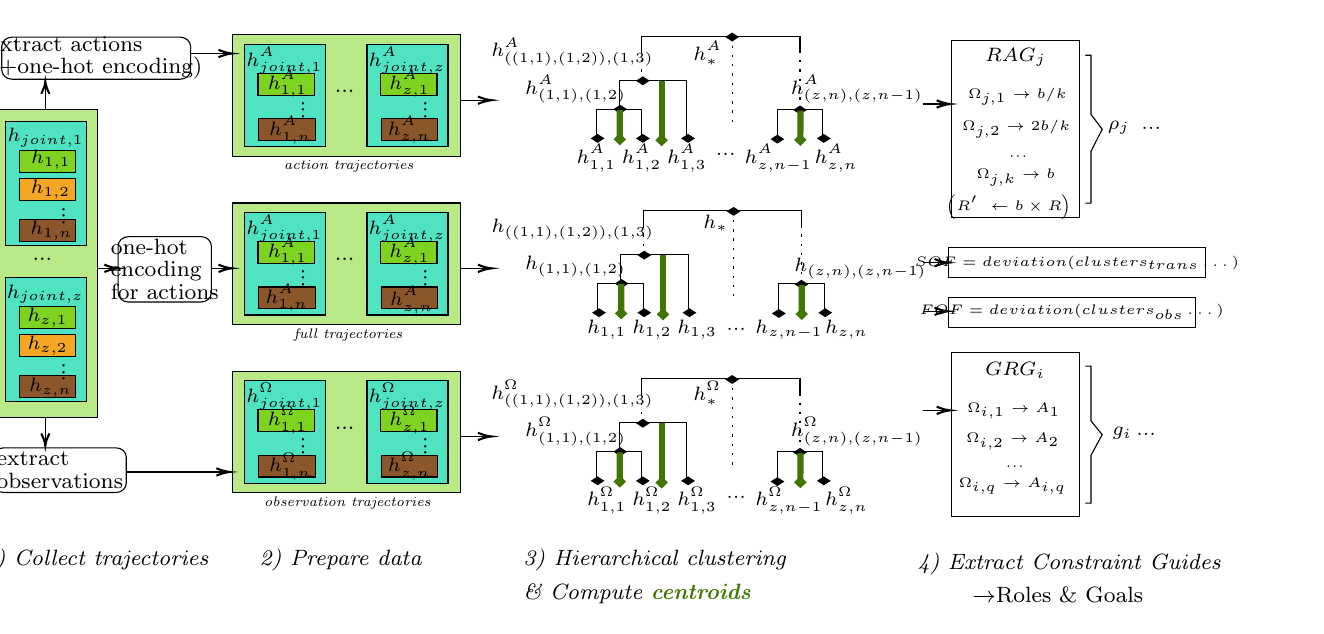
\begin{tikzpicture}[x=0.75pt,y=0.75pt,yscale=-0.9,xscale=1]
%uncomment if require: \path (0,1723); %set diagram left start at 0, and has height of 1723

\hspace{-0.6cm}

%Shape: Rectangle [id:dp09610487374035748] 
\draw  [fill={rgb, 255:red, 184; green, 233; blue, 134 }  ,fill opacity=1 ] (30,1232) -- (80,1232) -- (80,1397) -- (30,1397) -- cycle ;
%Shape: Rectangle [id:dp45316125392913] 
\draw  [fill={rgb, 255:red, 80; green, 227; blue, 194 }  ,fill opacity=1 ] (35.96,1238.4) -- (74.96,1238.4) -- (74.96,1304.76) -- (35.96,1304.76) -- cycle ;
%Shape: Rectangle [id:dp45830823192172254] 
\draw  [fill={rgb, 255:red, 245; green, 166; blue, 35 }  ,fill opacity=1 ] (42.44,1269.04) -- (69.69,1269.04) -- (69.69,1280.75) -- (42.44,1280.75) -- cycle ;
%Shape: Rectangle [id:dp3946596851341897] 
\draw  [fill={rgb, 255:red, 139; green, 87; blue, 42 }  ,fill opacity=1 ] (42.44,1290.91) -- (69.69,1290.91) -- (69.69,1302.62) -- (42.44,1302.62) -- cycle ;
%Shape: Rectangle [id:dp12555529945477895] 
\draw  [fill={rgb, 255:red, 126; green, 211; blue, 33 }  ,fill opacity=1 ] (42.44,1254.01) -- (69.69,1254.01) -- (69.69,1265.72) -- (42.44,1265.72) -- cycle ;
%Shape: Rectangle [id:dp7349415985100746] 
\draw  [fill={rgb, 255:red, 80; green, 227; blue, 194 }  ,fill opacity=1 ] (36,1322) -- (75,1322) -- (75,1388.37) -- (36,1388.37) -- cycle ;
%Shape: Rectangle [id:dp26642582947795324] 
\draw  [fill={rgb, 255:red, 245; green, 166; blue, 35 }  ,fill opacity=1 ] (42.48,1352.65) -- (69.72,1352.65) -- (69.72,1364.36) -- (42.48,1364.36) -- cycle ;
%Shape: Rectangle [id:dp9632684060086679] 
\draw  [fill={rgb, 255:red, 139; green, 87; blue, 42 }  ,fill opacity=1 ] (42.48,1374.51) -- (69.72,1374.51) -- (69.72,1386.22) -- (42.48,1386.22) -- cycle ;
%Shape: Rectangle [id:dp0008867618580383763] 
\draw  [fill={rgb, 255:red, 126; green, 211; blue, 33 }  ,fill opacity=1 ] (42.48,1337.62) -- (69.72,1337.62) -- (69.72,1349.33) -- (42.48,1349.33) -- cycle ;
%Shape: Rectangle [id:dp5049511033223727] 
\draw  [fill={rgb, 255:red, 255; green, 255; blue, 255 }  ,fill opacity=1 ] (30,1418.08) .. controls (30,1415.32) and (32.24,1413.08) .. (35,1413.08) -- (89,1413.08) .. controls (91.76,1413.08) and (94,1415.32) .. (94,1418.08) -- (94,1432) .. controls (94,1434.76) and (91.76,1437) .. (89,1437) -- (35,1437) .. controls (32.24,1437) and (30,1434.76) .. (30,1432) -- cycle ;

%Shape: Rectangle [id:dp861803318395177] 
\draw  [fill={rgb, 255:red, 184; green, 233; blue, 134 }  ,fill opacity=1 ] (145,1192) -- (255,1192) -- (255,1257) -- (145,1257) -- cycle ;
%Shape: Rectangle [id:dp6132217248920296] 
\draw  [fill={rgb, 255:red, 80; green, 227; blue, 194 }  ,fill opacity=1 ] (151,1197) -- (190,1197) -- (190,1252) -- (151,1252) -- cycle ;
%Shape: Rectangle [id:dp5733108309348334] 
\draw  [fill={rgb, 255:red, 139; green, 87; blue, 42 }  ,fill opacity=1 ] (157.76,1237) -- (185,1237) -- (185,1248.71) -- (157.76,1248.71) -- cycle ;
%Shape: Rectangle [id:dp2842929693852999] 
\draw  [fill={rgb, 255:red, 126; green, 211; blue, 33 }  ,fill opacity=1 ] (157.48,1212.62) -- (184.72,1212.62) -- (184.72,1224.33) -- (157.48,1224.33) -- cycle ;
%Shape: Rectangle [id:dp56024471923465] 
\draw  [fill={rgb, 255:red, 80; green, 227; blue, 194 }  ,fill opacity=1 ] (210,1197) -- (249,1197) -- (249,1252) -- (210,1252) -- cycle ;
%Shape: Rectangle [id:dp762658002129142] 
\draw  [fill={rgb, 255:red, 139; green, 87; blue, 42 }  ,fill opacity=1 ] (216.76,1237) -- (244,1237) -- (244,1248.71) -- (216.76,1248.71) -- cycle ;
%Shape: Rectangle [id:dp17126433901717386] 
\draw  [fill={rgb, 255:red, 126; green, 211; blue, 33 }  ,fill opacity=1 ] (216.48,1212.62) -- (243.72,1212.62) -- (243.72,1224.33) -- (216.48,1224.33) -- cycle ;
%Shape: Rectangle [id:dp9537774458308554] 
\draw  [fill={rgb, 255:red, 184; green, 233; blue, 134 }  ,fill opacity=1 ] (145,1372) -- (255,1372) -- (255,1437) -- (145,1437) -- cycle ;
%Shape: Rectangle [id:dp7233105184708959] 
\draw  [fill={rgb, 255:red, 80; green, 227; blue, 194 }  ,fill opacity=1 ] (151,1377) -- (190,1377) -- (190,1432) -- (151,1432) -- cycle ;
%Shape: Rectangle [id:dp6105572959886556] 
\draw  [fill={rgb, 255:red, 139; green, 87; blue, 42 }  ,fill opacity=1 ] (157.76,1417) -- (185,1417) -- (185,1428.71) -- (157.76,1428.71) -- cycle ;
%Shape: Rectangle [id:dp12021735107027742] 
\draw  [fill={rgb, 255:red, 126; green, 211; blue, 33 }  ,fill opacity=1 ] (157.48,1392.62) -- (184.72,1392.62) -- (184.72,1404.33) -- (157.48,1404.33) -- cycle ;
%Shape: Rectangle [id:dp013850868214046685] 
\draw  [fill={rgb, 255:red, 80; green, 227; blue, 194 }  ,fill opacity=1 ] (210,1377) -- (249,1377) -- (249,1432) -- (210,1432) -- cycle ;
%Shape: Rectangle [id:dp18055620205595135] 
\draw  [fill={rgb, 255:red, 139; green, 87; blue, 42 }  ,fill opacity=1 ] (216.76,1417) -- (244,1417) -- (244,1428.71) -- (216.76,1428.71) -- cycle ;
%Shape: Rectangle [id:dp8438669395198585] 
\draw  [fill={rgb, 255:red, 126; green, 211; blue, 33 }  ,fill opacity=1 ] (216.48,1392.62) -- (243.72,1392.62) -- (243.72,1404.33) -- (216.48,1404.33) -- cycle ;
%Straight Lines [id:da3008118547681833] 
\draw    (125,1202) -- (143,1202) ;
\draw [shift={(145,1202)}, rotate = 180] [color={rgb, 255:red, 0; green, 0; blue, 0 }  ][line width=0.75]    (6.56,-1.97) .. controls (4.17,-0.84) and (1.99,-0.18) .. (0,0) .. controls (1.99,0.18) and (4.17,0.84) .. (6.56,1.97)   ;
%Shape: Rectangle [id:dp31005292076420676] 
\draw  [fill={rgb, 255:red, 255; green, 255; blue, 255 }  ,fill opacity=1 ] (34,1198.24) .. controls (34,1195.48) and (36.24,1193.24) .. (39,1193.24) -- (120,1193.24) .. controls (122.76,1193.24) and (125,1195.48) .. (125,1198.24) -- (125,1210.76) .. controls (125,1213.52) and (122.76,1215.76) .. (120,1215.76) -- (39,1215.76) .. controls (36.24,1215.76) and (34,1213.52) .. (34,1210.76) -- cycle ;

%Straight Lines [id:da867093953960449] 
\draw    (55,1232) -- (55,1219) ;
\draw [shift={(55,1217)}, rotate = 90] [color={rgb, 255:red, 0; green, 0; blue, 0 }  ][line width=0.75]    (6.56,-1.97) .. controls (4.17,-0.84) and (1.99,-0.18) .. (0,0) .. controls (1.99,0.18) and (4.17,0.84) .. (6.56,1.97)   ;
%Straight Lines [id:da09509111300082773] 
\draw    (55,1397) -- (55,1410) ;
\draw [shift={(55,1412)}, rotate = 270] [color={rgb, 255:red, 0; green, 0; blue, 0 }  ][line width=0.75]    (6.56,-1.97) .. controls (4.17,-0.84) and (1.99,-0.18) .. (0,0) .. controls (1.99,0.18) and (4.17,0.84) .. (6.56,1.97)   ;
%Straight Lines [id:da37053818789319803] 
\draw    (320.53,1430.76) -- (320.53,1415.15) -- (342.33,1415.15) -- (342.33,1430.76) ;
%Straight Lines [id:da27331471605364943] 
\draw    (331.43,1415.15) -- (331.43,1399.53) -- (364.12,1399.53) -- (364.12,1430.76) ;
%Straight Lines [id:da4312567064966427] 
\draw    (342.33,1383.91) -- (342.33,1376.11) -- (418.61,1376.11) -- (418.61,1383.91) ;
%Straight Lines [id:da22888172465679524] 
\draw    (407.71,1430.76) -- (407.71,1415.15) -- (429.51,1415.15) -- (429.51,1430.76) ;
%Shape: Ellipse [id:dp6184217681327564] 
\draw  [line width=2.25]  (320.53,1430.76) .. controls (320.53,1430.55) and (320.78,1430.37) .. (321.08,1430.37) .. controls (321.38,1430.37) and (321.62,1430.55) .. (321.62,1430.76) .. controls (321.62,1430.98) and (321.38,1431.15) .. (321.08,1431.15) .. controls (320.78,1431.15) and (320.53,1430.98) .. (320.53,1430.76) -- cycle ;
%Shape: Ellipse [id:dp06577345173315474] 
\draw  [line width=2.25]  (342.33,1430.76) .. controls (342.33,1430.55) and (342.57,1430.37) .. (342.87,1430.37) .. controls (343.17,1430.37) and (343.42,1430.55) .. (343.42,1430.76) .. controls (343.42,1430.98) and (343.17,1431.15) .. (342.87,1431.15) .. controls (342.57,1431.15) and (342.33,1430.98) .. (342.33,1430.76) -- cycle ;
%Shape: Ellipse [id:dp7107422628707226] 
\draw  [line width=2.25]  (364.12,1430.76) .. controls (364.12,1430.55) and (364.37,1430.37) .. (364.67,1430.37) .. controls (364.97,1430.37) and (365.21,1430.55) .. (365.21,1430.76) .. controls (365.21,1430.98) and (364.97,1431.15) .. (364.67,1431.15) .. controls (364.37,1431.15) and (364.12,1430.98) .. (364.12,1430.76) -- cycle ;
%Shape: Ellipse [id:dp6939382648562396] 
\draw  [line width=2.25]  (407.17,1431.15) .. controls (407.17,1430.94) and (407.41,1430.76) .. (407.71,1430.76) .. controls (408.01,1430.76) and (408.26,1430.94) .. (408.26,1431.15) .. controls (408.26,1431.37) and (408.01,1431.54) .. (407.71,1431.54) .. controls (407.41,1431.54) and (407.17,1431.37) .. (407.17,1431.15) -- cycle ;
%Shape: Ellipse [id:dp08118677913158812] 
\draw  [line width=2.25]  (429.51,1430.76) .. controls (429.51,1430.55) and (429.75,1430.37) .. (430.05,1430.37) .. controls (430.35,1430.37) and (430.6,1430.55) .. (430.6,1430.76) .. controls (430.6,1430.98) and (430.35,1431.15) .. (430.05,1431.15) .. controls (429.75,1431.15) and (429.51,1430.98) .. (429.51,1430.76) -- cycle ;
%Shape: Ellipse [id:dp9493188068363742] 
\draw  [line width=2.25]  (331.43,1415.15) .. controls (331.43,1414.93) and (331.67,1414.75) .. (331.97,1414.75) .. controls (332.27,1414.75) and (332.52,1414.93) .. (332.52,1415.15) .. controls (332.52,1415.36) and (332.27,1415.54) .. (331.97,1415.54) .. controls (331.67,1415.54) and (331.43,1415.36) .. (331.43,1415.15) -- cycle ;
%Shape: Ellipse [id:dp31776400962313445] 
\draw  [line width=2.25]  (342.33,1399.92) .. controls (342.33,1399.7) and (342.57,1399.53) .. (342.87,1399.53) .. controls (343.17,1399.53) and (343.42,1399.7) .. (343.42,1399.92) .. controls (343.42,1400.14) and (343.17,1400.31) .. (342.87,1400.31) .. controls (342.57,1400.31) and (342.33,1400.14) .. (342.33,1399.92) -- cycle ;
%Shape: Ellipse [id:dp156886046038465] 
\draw  [line width=2.25]  (385.37,1376.5) .. controls (385.37,1376.28) and (385.62,1376.11) .. (385.92,1376.11) .. controls (386.22,1376.11) and (386.46,1376.28) .. (386.46,1376.5) .. controls (386.46,1376.71) and (386.22,1376.89) .. (385.92,1376.89) .. controls (385.62,1376.89) and (385.37,1376.71) .. (385.37,1376.5) -- cycle ;
%Shape: Ellipse [id:dp4090467774188007] 
\draw  [line width=2.25]  (418.06,1415.54) .. controls (418.06,1415.32) and (418.31,1415.15) .. (418.61,1415.15) .. controls (418.91,1415.15) and (419.15,1415.32) .. (419.15,1415.54) .. controls (419.15,1415.75) and (418.91,1415.93) .. (418.61,1415.93) .. controls (418.31,1415.93) and (418.06,1415.75) .. (418.06,1415.54) -- cycle ;
%Straight Lines [id:da5835970444465544] 
\draw  [dash pattern={on 0.84pt off 2.51pt}]  (342.33,1383.91) -- (342.33,1399.53) ;
%Straight Lines [id:da1689158486837592] 
\draw  [dash pattern={on 0.84pt off 2.51pt}]  (418.61,1383.91) -- (418.61,1415.15) ;
%Straight Lines [id:da2070689850273354] 
\draw  [dash pattern={on 0.84pt off 2.51pt}]  (385.92,1376.11) -- (385.92,1422.95) ;
%Straight Lines [id:da21678640379690228] 
\draw    (321.22,1340.76) -- (321.22,1325.15) -- (343.02,1325.15) -- (343.02,1340.76) ;
%Straight Lines [id:da3653267745057789] 
\draw    (332.12,1325.15) -- (332.12,1309.53) -- (364.81,1309.53) -- (364.81,1340.76) ;
%Straight Lines [id:da9487811381350612] 
\draw    (343.02,1293.91) -- (343.02,1286.11) -- (419.3,1286.11) -- (419.3,1293.91) ;
%Straight Lines [id:da6273772791005832] 
\draw    (408.4,1340.76) -- (408.4,1325.15) -- (430.2,1325.15) -- (430.2,1340.76) ;
%Shape: Ellipse [id:dp361908442745964] 
\draw  [line width=2.25]  (321.22,1340.76) .. controls (321.22,1340.55) and (321.47,1340.37) .. (321.77,1340.37) .. controls (322.07,1340.37) and (322.31,1340.55) .. (322.31,1340.76) .. controls (322.31,1340.98) and (322.07,1341.15) .. (321.77,1341.15) .. controls (321.47,1341.15) and (321.22,1340.98) .. (321.22,1340.76) -- cycle ;
%Shape: Ellipse [id:dp34035499911302736] 
\draw  [line width=2.25]  (343.02,1340.76) .. controls (343.02,1340.55) and (343.26,1340.37) .. (343.56,1340.37) .. controls (343.87,1340.37) and (344.11,1340.55) .. (344.11,1340.76) .. controls (344.11,1340.98) and (343.87,1341.15) .. (343.56,1341.15) .. controls (343.26,1341.15) and (343.02,1340.98) .. (343.02,1340.76) -- cycle ;
%Shape: Ellipse [id:dp8093356810114974] 
\draw  [line width=2.25]  (364.81,1340.76) .. controls (364.81,1340.55) and (365.06,1340.37) .. (365.36,1340.37) .. controls (365.66,1340.37) and (365.9,1340.55) .. (365.9,1340.76) .. controls (365.9,1340.98) and (365.66,1341.15) .. (365.36,1341.15) .. controls (365.06,1341.15) and (364.81,1340.98) .. (364.81,1340.76) -- cycle ;
%Shape: Ellipse [id:dp6886301228573949] 
\draw  [line width=2.25]  (407.86,1341.15) .. controls (407.86,1340.94) and (408.1,1340.76) .. (408.4,1340.76) .. controls (408.71,1340.76) and (408.95,1340.94) .. (408.95,1341.15) .. controls (408.95,1341.37) and (408.71,1341.54) .. (408.4,1341.54) .. controls (408.1,1341.54) and (407.86,1341.37) .. (407.86,1341.15) -- cycle ;
%Shape: Ellipse [id:dp6104880437237735] 
\draw  [line width=2.25]  (430.2,1340.76) .. controls (430.2,1340.55) and (430.44,1340.37) .. (430.74,1340.37) .. controls (431.05,1340.37) and (431.29,1340.55) .. (431.29,1340.76) .. controls (431.29,1340.98) and (431.05,1341.15) .. (430.74,1341.15) .. controls (430.44,1341.15) and (430.2,1340.98) .. (430.2,1340.76) -- cycle ;
%Shape: Ellipse [id:dp3847126134177271] 
\draw  [line width=2.25]  (332.12,1325.15) .. controls (332.12,1324.93) and (332.37,1324.75) .. (332.67,1324.75) .. controls (332.97,1324.75) and (333.21,1324.93) .. (333.21,1325.15) .. controls (333.21,1325.36) and (332.97,1325.54) .. (332.67,1325.54) .. controls (332.37,1325.54) and (332.12,1325.36) .. (332.12,1325.15) -- cycle ;
%Shape: Ellipse [id:dp9172247745940925] 
\draw  [line width=2.25]  (343.02,1309.92) .. controls (343.02,1309.7) and (343.26,1309.53) .. (343.56,1309.53) .. controls (343.87,1309.53) and (344.11,1309.7) .. (344.11,1309.92) .. controls (344.11,1310.14) and (343.87,1310.31) .. (343.56,1310.31) .. controls (343.26,1310.31) and (343.02,1310.14) .. (343.02,1309.92) -- cycle ;
%Shape: Ellipse [id:dp4031282586521814] 
\draw  [line width=2.25]  (386.06,1286.5) .. controls (386.06,1286.28) and (386.31,1286.11) .. (386.61,1286.11) .. controls (386.91,1286.11) and (387.15,1286.28) .. (387.15,1286.5) .. controls (387.15,1286.71) and (386.91,1286.89) .. (386.61,1286.89) .. controls (386.31,1286.89) and (386.06,1286.71) .. (386.06,1286.5) -- cycle ;
%Shape: Ellipse [id:dp010476775151872508] 
\draw  [line width=2.25]  (418.76,1325.54) .. controls (418.76,1325.32) and (419,1325.15) .. (419.3,1325.15) .. controls (419.6,1325.15) and (419.85,1325.32) .. (419.85,1325.54) .. controls (419.85,1325.75) and (419.6,1325.93) .. (419.3,1325.93) .. controls (419,1325.93) and (418.76,1325.75) .. (418.76,1325.54) -- cycle ;
%Straight Lines [id:da6762017945408133] 
\draw  [dash pattern={on 0.84pt off 2.51pt}]  (343.02,1293.91) -- (343.02,1309.53) ;
%Straight Lines [id:da9097085331303272] 
\draw  [dash pattern={on 0.84pt off 2.51pt}]  (419.3,1293.91) -- (419.3,1325.15) ;
%Straight Lines [id:da20995347959711252] 
\draw  [dash pattern={on 0.84pt off 2.51pt}]  (386.61,1286.11) -- (386.61,1332.95) ;
%Straight Lines [id:da300589271672265] 
\draw    (320.53,1247.44) -- (320.53,1231.82) -- (342.33,1231.82) -- (342.33,1247.44) ;
%Straight Lines [id:da7941749924863761] 
\draw    (331.43,1231.82) -- (331.43,1216.21) -- (364.12,1216.21) -- (364.12,1247.44) ;
%Straight Lines [id:da036984986996662195] 
\draw    (342.33,1200.59) -- (342.33,1192.78) -- (418.61,1192.78) -- (418.61,1200.59) ;
%Straight Lines [id:da2521545303562105] 
\draw    (407.71,1247.44) -- (407.71,1231.82) -- (429.51,1231.82) -- (429.51,1247.44) ;
%Shape: Ellipse [id:dp8674458972711949] 
\draw  [line width=2.25]  (320.53,1247.44) .. controls (320.53,1247.22) and (320.78,1247.05) .. (321.08,1247.05) .. controls (321.38,1247.05) and (321.62,1247.22) .. (321.62,1247.44) .. controls (321.62,1247.66) and (321.38,1247.83) .. (321.08,1247.83) .. controls (320.78,1247.83) and (320.53,1247.66) .. (320.53,1247.44) -- cycle ;
%Shape: Ellipse [id:dp40445696985977] 
\draw  [line width=2.25]  (342.33,1247.44) .. controls (342.33,1247.22) and (342.57,1247.05) .. (342.87,1247.05) .. controls (343.17,1247.05) and (343.42,1247.22) .. (343.42,1247.44) .. controls (343.42,1247.66) and (343.17,1247.83) .. (342.87,1247.83) .. controls (342.57,1247.83) and (342.33,1247.66) .. (342.33,1247.44) -- cycle ;
%Shape: Ellipse [id:dp9379775866500679] 
\draw  [line width=2.25]  (364.12,1247.44) .. controls (364.12,1247.22) and (364.37,1247.05) .. (364.67,1247.05) .. controls (364.97,1247.05) and (365.21,1247.22) .. (365.21,1247.44) .. controls (365.21,1247.66) and (364.97,1247.83) .. (364.67,1247.83) .. controls (364.37,1247.83) and (364.12,1247.66) .. (364.12,1247.44) -- cycle ;
%Shape: Ellipse [id:dp9822823316274046] 
\draw  [line width=2.25]  (407.17,1247.83) .. controls (407.17,1247.61) and (407.41,1247.44) .. (407.71,1247.44) .. controls (408.01,1247.44) and (408.26,1247.61) .. (408.26,1247.83) .. controls (408.26,1248.05) and (408.01,1248.22) .. (407.71,1248.22) .. controls (407.41,1248.22) and (407.17,1248.05) .. (407.17,1247.83) -- cycle ;
%Shape: Ellipse [id:dp2170044467275838] 
\draw  [line width=2.25]  (429.51,1247.44) .. controls (429.51,1247.22) and (429.75,1247.05) .. (430.05,1247.05) .. controls (430.35,1247.05) and (430.6,1247.22) .. (430.6,1247.44) .. controls (430.6,1247.66) and (430.35,1247.83) .. (430.05,1247.83) .. controls (429.75,1247.83) and (429.51,1247.66) .. (429.51,1247.44) -- cycle ;
%Shape: Ellipse [id:dp9651952068892246] 
\draw  [line width=2.25]  (331.43,1231.82) .. controls (331.43,1231.61) and (331.67,1231.43) .. (331.97,1231.43) .. controls (332.27,1231.43) and (332.52,1231.61) .. (332.52,1231.82) .. controls (332.52,1232.04) and (332.27,1232.21) .. (331.97,1232.21) .. controls (331.67,1232.21) and (331.43,1232.04) .. (331.43,1231.82) -- cycle ;
%Shape: Ellipse [id:dp13471864298862868] 
\draw  [line width=2.25]  (342.33,1216.6) .. controls (342.33,1216.38) and (342.57,1216.21) .. (342.87,1216.21) .. controls (343.17,1216.21) and (343.42,1216.38) .. (343.42,1216.6) .. controls (343.42,1216.81) and (343.17,1216.99) .. (342.87,1216.99) .. controls (342.57,1216.99) and (342.33,1216.81) .. (342.33,1216.6) -- cycle ;
%Shape: Ellipse [id:dp5352955294705005] 
\draw  [line width=2.25]  (385.37,1193.17) .. controls (385.37,1192.96) and (385.62,1192.78) .. (385.92,1192.78) .. controls (386.22,1192.78) and (386.46,1192.96) .. (386.46,1193.17) .. controls (386.46,1193.39) and (386.22,1193.57) .. (385.92,1193.57) .. controls (385.62,1193.57) and (385.37,1193.39) .. (385.37,1193.17) -- cycle ;
%Shape: Ellipse [id:dp3936416877844342] 
\draw  [line width=2.25]  (418.06,1232.21) .. controls (418.06,1232) and (418.31,1231.82) .. (418.61,1231.82) .. controls (418.91,1231.82) and (419.15,1232) .. (419.15,1232.21) .. controls (419.15,1232.43) and (418.91,1232.6) .. (418.61,1232.6) .. controls (418.31,1232.6) and (418.06,1232.43) .. (418.06,1232.21) -- cycle ;
%Straight Lines [id:da25854309643003515] 
\draw  [dash pattern={on 0.84pt off 2.51pt}]  (342.33,1200.59) -- (342.33,1216.21) ;
%Straight Lines [id:da7455747836351959] 
\draw  [dash pattern={on 0.84pt off 2.51pt}]  (418.61,1200.59) -- (418.61,1231.82) ;
%Straight Lines [id:da12353776549987561] 
\draw  [dash pattern={on 0.84pt off 2.51pt}]  (385.92,1192.78) -- (385.92,1239.63) ;
%Straight Lines [id:da4513495950780275] 
\draw    (94,1426) -- (136.2,1426) -- (142,1426) ;
\draw [shift={(144,1426)}, rotate = 180] [color={rgb, 255:red, 0; green, 0; blue, 0 }  ][line width=0.75]    (6.56,-1.97) .. controls (4.17,-0.84) and (1.99,-0.18) .. (0,0) .. controls (1.99,0.18) and (4.17,0.84) .. (6.56,1.97)   ;
%Shape: Rectangle [id:dp2785184585505095] 
\draw  [fill={rgb, 255:red, 184; green, 233; blue, 134 }  ,fill opacity=1 ] (145,1282) -- (255,1282) -- (255,1347) -- (145,1347) -- cycle ;
%Shape: Rectangle [id:dp9389588556238666] 
\draw  [fill={rgb, 255:red, 80; green, 227; blue, 194 }  ,fill opacity=1 ] (151,1287) -- (190,1287) -- (190,1342) -- (151,1342) -- cycle ;
%Shape: Rectangle [id:dp4298482952175806] 
\draw  [fill={rgb, 255:red, 139; green, 87; blue, 42 }  ,fill opacity=1 ] (157.76,1327) -- (185,1327) -- (185,1338.71) -- (157.76,1338.71) -- cycle ;
%Shape: Rectangle [id:dp17841550147931018] 
\draw  [fill={rgb, 255:red, 126; green, 211; blue, 33 }  ,fill opacity=1 ] (157.48,1302.62) -- (184.72,1302.62) -- (184.72,1314.33) -- (157.48,1314.33) -- cycle ;
%Shape: Rectangle [id:dp6094565240843841] 
\draw  [fill={rgb, 255:red, 80; green, 227; blue, 194 }  ,fill opacity=1 ] (210,1287) -- (249,1287) -- (249,1342) -- (210,1342) -- cycle ;
%Shape: Rectangle [id:dp8602093968638864] 
\draw  [fill={rgb, 255:red, 139; green, 87; blue, 42 }  ,fill opacity=1 ] (216.76,1327) -- (244,1327) -- (244,1338.71) -- (216.76,1338.71) -- cycle ;
%Shape: Rectangle [id:dp4790153776177223] 
\draw  [fill={rgb, 255:red, 126; green, 211; blue, 33 }  ,fill opacity=1 ] (216.48,1302.62) -- (243.72,1302.62) -- (243.72,1314.33) -- (216.48,1314.33) -- cycle ;
%Shape: Rectangle [id:dp22809977923512426] 
\draw  [fill={rgb, 255:red, 255; green, 255; blue, 255 }  ,fill opacity=1 ] (90.08,1305.03) .. controls (90.08,1302.27) and (92.32,1300.03) .. (95.08,1300.03) -- (130,1300.03) .. controls (132.76,1300.03) and (135,1302.27) .. (135,1305.03) -- (135,1330.03) .. controls (135,1332.79) and (132.76,1335.03) .. (130,1335.03) -- (95.08,1335.03) .. controls (92.32,1335.03) and (90.08,1332.79) .. (90.08,1330.03) -- cycle ;

%Straight Lines [id:da9452281321416813] 
\draw    (80,1317) -- (88,1317) ;
\draw [shift={(90,1317)}, rotate = 180] [color={rgb, 255:red, 0; green, 0; blue, 0 }  ][line width=0.75]    (6.56,-1.97) .. controls (4.17,-0.84) and (1.99,-0.18) .. (0,0) .. controls (1.99,0.18) and (4.17,0.84) .. (6.56,1.97)   ;
%Straight Lines [id:da2944197005580337] 
\draw    (135,1317) -- (143,1317) ;
\draw [shift={(145,1317)}, rotate = 180] [color={rgb, 255:red, 0; green, 0; blue, 0 }  ][line width=0.75]    (6.56,-1.97) .. controls (4.17,-0.84) and (1.99,-0.18) .. (0,0) .. controls (1.99,0.18) and (4.17,0.84) .. (6.56,1.97)   ;
%Straight Lines [id:da6740194662301707] 
\draw    (255,1317) -- (268,1317) ;
\draw [shift={(270,1317)}, rotate = 180] [color={rgb, 255:red, 0; green, 0; blue, 0 }  ][line width=0.75]    (6.56,-1.97) .. controls (4.17,-0.84) and (1.99,-0.18) .. (0,0) .. controls (1.99,0.18) and (4.17,0.84) .. (6.56,1.97)   ;
%Straight Lines [id:da005500304853916171] 
\draw    (255,1407) -- (268,1407) ;
\draw [shift={(270,1407)}, rotate = 180] [color={rgb, 255:red, 0; green, 0; blue, 0 }  ][line width=0.75]    (6.56,-1.97) .. controls (4.17,-0.84) and (1.99,-0.18) .. (0,0) .. controls (1.99,0.18) and (4.17,0.84) .. (6.56,1.97)   ;
%Straight Lines [id:da8722725448495506] 
\draw    (255,1227) -- (268,1227) ;
\draw [shift={(270,1227)}, rotate = 180] [color={rgb, 255:red, 0; green, 0; blue, 0 }  ][line width=0.75]    (6.56,-1.97) .. controls (4.17,-0.84) and (1.99,-0.18) .. (0,0) .. controls (1.99,0.18) and (4.17,0.84) .. (6.56,1.97)   ;
%Straight Lines [id:da8904876996863923] 
\draw [color={rgb, 255:red, 65; green, 117; blue, 5 }  ,draw opacity=1 ][line width=2.25]    (331.77,1432.09) -- (331.81,1415.54) ;
%Shape: Ellipse [id:dp8844330156287957] 
\draw  [color={rgb, 255:red, 65; green, 117; blue, 5 }  ,draw opacity=1 ][line width=2.25]  (330.92,1431.18) .. controls (330.92,1430.67) and (331.3,1430.26) .. (331.77,1430.26) .. controls (332.24,1430.26) and (332.63,1430.67) .. (332.63,1431.18) .. controls (332.63,1431.68) and (332.24,1432.09) .. (331.77,1432.09) .. controls (331.3,1432.09) and (330.92,1431.68) .. (330.92,1431.18) -- cycle ;
%Straight Lines [id:da22885587580730704] 
\draw [color={rgb, 255:red, 65; green, 117; blue, 5 }  ,draw opacity=1 ][line width=2.25]    (351.94,1430.76) -- (351.94,1399.93) ;
%Shape: Ellipse [id:dp6292633385955162] 
\draw  [color={rgb, 255:red, 65; green, 117; blue, 5 }  ,draw opacity=1 ][line width=2.25]  (351.08,1431.68) .. controls (351.08,1431.17) and (351.47,1430.76) .. (351.94,1430.76) .. controls (352.41,1430.76) and (352.79,1431.17) .. (352.79,1431.68) .. controls (352.79,1432.18) and (352.41,1432.59) .. (351.94,1432.59) .. controls (351.47,1432.59) and (351.08,1432.18) .. (351.08,1431.68) -- cycle ;
%Straight Lines [id:da8887764774403707] 
\draw [color={rgb, 255:red, 65; green, 117; blue, 5 }  ,draw opacity=1 ][line width=2.25]    (418.77,1432.43) -- (418.81,1415.87) ;
%Shape: Ellipse [id:dp2510234130651231] 
\draw  [color={rgb, 255:red, 65; green, 117; blue, 5 }  ,draw opacity=1 ][line width=2.25]  (417.92,1431.51) .. controls (417.92,1431) and (418.3,1430.59) .. (418.77,1430.59) .. controls (419.24,1430.59) and (419.63,1431) .. (419.63,1431.51) .. controls (419.63,1432.01) and (419.24,1432.43) .. (418.77,1432.43) .. controls (418.3,1432.43) and (417.92,1432.01) .. (417.92,1431.51) -- cycle ;
%Straight Lines [id:da6067776943388129] 
\draw [color={rgb, 255:red, 65; green, 117; blue, 5 }  ,draw opacity=1 ][line width=2.25]    (332.44,1342.05) -- (332.47,1325.49) ;
%Shape: Ellipse [id:dp5699447742396252] 
\draw  [color={rgb, 255:red, 65; green, 117; blue, 5 }  ,draw opacity=1 ][line width=2.25]  (331.58,1341.13) .. controls (331.58,1340.62) and (331.97,1340.21) .. (332.44,1340.21) .. controls (332.91,1340.21) and (333.29,1340.62) .. (333.29,1341.13) .. controls (333.29,1341.64) and (332.91,1342.05) .. (332.44,1342.05) .. controls (331.97,1342.05) and (331.58,1341.64) .. (331.58,1341.13) -- cycle ;
%Straight Lines [id:da5298186005386079] 
\draw [color={rgb, 255:red, 65; green, 117; blue, 5 }  ,draw opacity=1 ][line width=2.25]    (352.61,1340.71) -- (352.61,1309.88) ;
%Shape: Ellipse [id:dp2450820398379311] 
\draw  [color={rgb, 255:red, 65; green, 117; blue, 5 }  ,draw opacity=1 ][line width=2.25]  (351.75,1341.63) .. controls (351.75,1341.12) and (352.13,1340.71) .. (352.61,1340.71) .. controls (353.08,1340.71) and (353.46,1341.12) .. (353.46,1341.63) .. controls (353.46,1342.14) and (353.08,1342.55) .. (352.61,1342.55) .. controls (352.13,1342.55) and (351.75,1342.14) .. (351.75,1341.63) -- cycle ;
%Straight Lines [id:da14297003928812257] 
\draw [color={rgb, 255:red, 65; green, 117; blue, 5 }  ,draw opacity=1 ][line width=2.25]    (419.44,1342.38) -- (419.47,1325.82) ;
%Shape: Ellipse [id:dp9917626268001508] 
\draw  [color={rgb, 255:red, 65; green, 117; blue, 5 }  ,draw opacity=1 ][line width=2.25]  (418.58,1341.46) .. controls (418.58,1340.96) and (418.97,1340.55) .. (419.44,1340.55) .. controls (419.91,1340.55) and (420.29,1340.96) .. (420.29,1341.46) .. controls (420.29,1341.97) and (419.91,1342.38) .. (419.44,1342.38) .. controls (418.97,1342.38) and (418.58,1341.97) .. (418.58,1341.46) -- cycle ;
%Straight Lines [id:da596053750216235] 
\draw [color={rgb, 255:red, 65; green, 117; blue, 5 }  ,draw opacity=1 ][line width=2.25]    (331.77,1248.83) -- (331.81,1232.28) ;
%Shape: Ellipse [id:dp8751972343270811] 
\draw  [color={rgb, 255:red, 65; green, 117; blue, 5 }  ,draw opacity=1 ][line width=2.25]  (330.92,1247.92) .. controls (330.92,1247.41) and (331.3,1247) .. (331.77,1247) .. controls (332.24,1247) and (332.63,1247.41) .. (332.63,1247.92) .. controls (332.63,1248.42) and (332.24,1248.83) .. (331.77,1248.83) .. controls (331.3,1248.83) and (330.92,1248.42) .. (330.92,1247.92) -- cycle ;
%Straight Lines [id:da7739385062504773] 
\draw [color={rgb, 255:red, 65; green, 117; blue, 5 }  ,draw opacity=1 ][line width=2.25]    (351.94,1247.5) -- (351.94,1216.67) ;
%Shape: Ellipse [id:dp9654136677444494] 
\draw  [color={rgb, 255:red, 65; green, 117; blue, 5 }  ,draw opacity=1 ][line width=2.25]  (351.08,1248.42) .. controls (351.08,1247.91) and (351.47,1247.5) .. (351.94,1247.5) .. controls (352.41,1247.5) and (352.79,1247.91) .. (352.79,1248.42) .. controls (352.79,1248.92) and (352.41,1249.33) .. (351.94,1249.33) .. controls (351.47,1249.33) and (351.08,1248.92) .. (351.08,1248.42) -- cycle ;
%Straight Lines [id:da6806437518594021] 
\draw [color={rgb, 255:red, 65; green, 117; blue, 5 }  ,draw opacity=1 ][line width=2.25]    (418.77,1249.17) -- (418.81,1232.61) ;
%Shape: Ellipse [id:dp3806348109693991] 
\draw  [color={rgb, 255:red, 65; green, 117; blue, 5 }  ,draw opacity=1 ][line width=2.25]  (417.92,1248.25) .. controls (417.92,1247.74) and (418.3,1247.33) .. (418.77,1247.33) .. controls (419.24,1247.33) and (419.63,1247.74) .. (419.63,1248.25) .. controls (419.63,1248.76) and (419.24,1249.17) .. (418.77,1249.17) .. controls (418.3,1249.17) and (417.92,1248.76) .. (417.92,1248.25) -- cycle ;
%Shape: Rectangle [id:dp6135707285093043] 
\draw   (491.61,1362) -- (553.43,1362) -- (553.43,1450.03) -- (491.61,1450.03) -- cycle ;
%Shape: Rectangle [id:dp595374667047198] 
\draw   (491.61,1195.03) -- (553.43,1195.03) -- (553.43,1290) -- (491.61,1290) -- cycle ;
%Straight Lines [id:da2554918433833141] 
\draw    (477.81,1393.03) -- (489,1393.03) ;
\draw [shift={(491,1393.03)}, rotate = 180] [color={rgb, 255:red, 0; green, 0; blue, 0 }  ][line width=0.75]    (6.56,-1.97) .. controls (4.17,-0.84) and (1.99,-0.18) .. (0,0) .. controls (1.99,0.18) and (4.17,0.84) .. (6.56,1.97)   ;
%Straight Lines [id:da11811337209895834] 
\draw    (477.81,1229.03) -- (489,1229.03) ;
\draw [shift={(491,1229.03)}, rotate = 180] [color={rgb, 255:red, 0; green, 0; blue, 0 }  ][line width=0.75]    (6.56,-1.97) .. controls (4.17,-0.84) and (1.99,-0.18) .. (0,0) .. controls (1.99,0.18) and (4.17,0.84) .. (6.56,1.97)   ;
%Straight Lines [id:da9318830602943007] 
\draw    (556.12,1202.94) -- (558.81,1202.94) -- (558.81,1234.6) -- (564.18,1242.52) -- (558.81,1254.39) -- (558.81,1282.09) -- (556.12,1282.09) ;
%Straight Lines [id:da8803930365580092] 
\draw    (556.12,1369.34) -- (558.81,1369.34) -- (558.81,1398.68) -- (564.18,1406.02) -- (558.81,1417.02) -- (558.81,1442.69) -- (556.12,1442.69) ;
%Straight Lines [id:da7173514032233753] 
\draw    (478,1314) -- (488,1314) ;
\draw [shift={(490,1314)}, rotate = 180] [color={rgb, 255:red, 0; green, 0; blue, 0 }  ][line width=0.75]    (6.56,-1.97) .. controls (4.17,-0.84) and (1.99,-0.18) .. (0,0) .. controls (1.99,0.18) and (4.17,0.84) .. (6.56,1.97)   ;
%Straight Lines [id:da05394772954338589] 
\draw    (478,1340) -- (488,1340) ;
\draw [shift={(490,1340)}, rotate = 180] [color={rgb, 255:red, 0; green, 0; blue, 0 }  ][line width=0.75]    (6.56,-1.97) .. controls (4.17,-0.84) and (1.99,-0.18) .. (0,0) .. controls (1.99,0.18) and (4.17,0.84) .. (6.56,1.97)   ;


% Text Node
\draw (585.36,1406) node  [font=\scriptsize] [align=left] {$\displaystyle ...$};
% Text Node
\draw    (490,1332.5) -- (609,1332.5) -- (609,1348.5) -- (490,1348.5) -- cycle  ;
\draw (549.5,1340.5) node  [font=\tiny] [align=left] {$\displaystyle FOF=deviation( clusters_{obs} \dotsc )$};
% Text Node
\draw    (490,1306) -- (614,1306) -- (614,1322) -- (490,1322) -- cycle  ;
\draw (552,1314) node  [font=\tiny] [align=left] {$\displaystyle SOF=deviation( clusters_{trans} \dotsc )$};
% Text Node
\draw (572.19,1241.72) node  [font=\scriptsize] [align=left] {$\displaystyle \rho _{j}$};
% Text Node
\draw (587.83,1242) node  [font=\scriptsize] [align=left] {$\displaystyle ...$};
% Text Node
\draw (573.83,1405.28) node  [font=\scriptsize] [align=left] {$\displaystyle g_{i}$};
% Text Node
\draw (519.41,1284.34) node  [font=\tiny] [align=left] {$\displaystyle \left( R'\ \leftarrow b\times R\right)$};
% Text Node
\draw (523.69,1256.98) node  [font=\tiny] [align=left] {$\displaystyle ...$};
% Text Node
\draw (522.59,1268.24) node  [font=\tiny] [align=left] {$\displaystyle \Omega _{j,k}\rightarrow b$};
% Text Node
\draw (522.79,1242.61) node  [font=\tiny] [align=left] {$\displaystyle \Omega _{j,2}\rightarrow 2b/k$};
% Text Node
\draw (523.33,1225.08) node  [font=\tiny] [align=left] {$\displaystyle \Omega _{j,1}\rightarrow b/k$};
% Text Node
\draw (522.08,1423.09) node  [font=\tiny] [align=left] {$\displaystyle ...$};
% Text Node
\draw (520.98,1433.52) node  [font=\tiny] [align=left] {$\displaystyle \Omega _{i,q}\rightarrow A_{i,q}$};
% Text Node
\draw (521.18,1409.77) node  [font=\tiny] [align=left] {$\displaystyle \Omega _{i,2}\rightarrow A_{2}$};
% Text Node
\draw (521.71,1393.52) node  [font=\tiny] [align=left] {$\displaystyle \Omega _{i,1}\rightarrow A_{1}$};
% Text Node
\draw (522.22,1371.84) node  [font=\scriptsize] [align=left] {$\displaystyle GRG_{i}$};
% Text Node
\draw (522.5,1204) node  [font=\scriptsize] [align=left] {$\displaystyle RAG_{j}$};
% Text Node
\draw (201.18,1352.5) node   [align=left] {{\tiny \textit{full trajectories}}};
% Text Node
\draw (200.77,1442.5) node   [align=left] {{\tiny \textit{observation trajectories}}};
% Text Node
\draw (201.39,1262.5) node   [align=left] {{\tiny \textit{action trajectories}}};
% Text Node
\draw (189.99,1313.53) node [anchor=west] [inner sep=0.75pt]  [font=\footnotesize] [align=left] {\begin{minipage}[lt]{9.53pt}\setlength\topsep{0pt}
\begin{flushright}
...
\end{flushright}

\end{minipage}};
% Text Node
\draw (231.5,1334.03) node  [font=\scriptsize] [align=left] {$\displaystyle h_{z,n}^{A}$};
% Text Node
\draw (230.45,1308.24) node  [font=\scriptsize] [align=left] {$\displaystyle h_{z,1}^{A}$};
% Text Node
\draw (229.23,1295.83) node  [font=\scriptsize] [align=left] {$\displaystyle h_{joint,z}^{A}$};
% Text Node
\draw (240,1312) node [anchor=north west][inner sep=0.75pt]  [font=\footnotesize,rotate=-90] [align=left] {\begin{minipage}[lt]{9.53pt}\setlength\topsep{0pt}
\begin{flushright}
...
\end{flushright}

\end{minipage}};
% Text Node
\draw (171.38,1332.86) node  [font=\scriptsize] [align=left] {$\displaystyle h_{1,n}^{A}$};
% Text Node
\draw (171.69,1308.24) node  [font=\scriptsize] [align=left] {$\displaystyle h_{1,1}^{A}$};
% Text Node
\draw (170.22,1295.83) node  [font=\scriptsize] [align=left] {$\displaystyle h_{joint,1}^{A}$};
% Text Node
\draw (181,1312) node [anchor=north west][inner sep=0.75pt]  [font=\footnotesize,rotate=-90] [align=left] {\begin{minipage}[lt]{9.53pt}\setlength\topsep{0pt}
\begin{flushright}
...
\end{flushright}

\end{minipage}};
% Text Node
\draw (474,1468.03) node [anchor=north west][inner sep=0.75pt]   [align=left] {{\footnotesize \textit{4) Extract Constraint Guides}}\\{\footnotesize  \ \ \ \ \ \ \ $\displaystyle \rightarrow $Roles \& Goals}};
% Text Node
\draw (284,1466) node [anchor=north west][inner sep=0.75pt]   [align=left] {{\footnotesize \textit{3) Hierarchical clustering}}\\{\footnotesize \textit{\& Compute \textcolor[rgb]{0.25,0.46,0.02}{\textbf{centroids}}}}};
% Text Node
\draw (157,1466) node [anchor=north west][inner sep=0.75pt]   [align=left] {{\footnotesize \textit{2) Prepare data}}};
% Text Node
\draw (24,1466) node [anchor=north west][inner sep=0.75pt]   [align=left] {{\footnotesize \textit{1) Collect trajectories}}};
% Text Node
\draw (446,1221.03) node  [font=\scriptsize] [align=left] {$\displaystyle h_{( z,n) ,( z,n-1)}^{A}$};
% Text Node
\draw (366,1194.03) node [anchor=north west][inner sep=0.75pt]  [font=\scriptsize] [align=left] {$\displaystyle h_{*}^{A}$};
% Text Node
\draw (309,1201.03) node  [font=\scriptsize] [align=left] {$\displaystyle h_{(( 1,1) ,( 1,2)) ,( 1,3)}^{A}$};
% Text Node
\draw (310.5,1221.03) node  [font=\scriptsize] [align=left] {$\displaystyle h_{( 1,1) ,( 1,2)}^{A}$};
% Text Node
\draw (436.01,1258) node  [font=\scriptsize] [align=left] {$\displaystyle h_{z,n}^{A}$};
% Text Node
\draw (408.15,1258) node  [font=\scriptsize] [align=left] {$\displaystyle h_{z,n-1}^{A}$};
% Text Node
\draw (382.82,1256.24) node  [font=\scriptsize] [align=left] {$\displaystyle ...$};
% Text Node
\draw (364.09,1258) node  [font=\scriptsize] [align=left] {$\displaystyle h_{1,3}^{A}$};
% Text Node
\draw (342.3,1258) node  [font=\scriptsize] [align=left] {$\displaystyle h_{1,2}^{A}$};
% Text Node
\draw (320.5,1258) node  [font=\scriptsize] [align=left] {$\displaystyle h_{1,1}^{A}$};
% Text Node
\draw (446,1404.35) node  [font=\scriptsize] [align=left] {$\displaystyle h_{( z,n) ,( z,n-1)}^{\Omega }$};
% Text Node
\draw (366,1376.03) node [anchor=north west][inner sep=0.75pt]  [font=\scriptsize] [align=left] {$\displaystyle h_{*}^{\Omega }$};
% Text Node
\draw (309,1384.35) node  [font=\scriptsize] [align=left] {$\displaystyle h_{(( 1,1) ,( 1,2)) ,( 1,3)}^{\Omega }$};
% Text Node
\draw (310.5,1404.35) node  [font=\scriptsize] [align=left] {$\displaystyle h_{( 1,1) ,( 1,2)}^{\Omega }$};
% Text Node
\draw (441.01,1441.26) node  [font=\scriptsize] [align=left] {$\displaystyle h_{z,n}^{\Omega }$};
% Text Node
\draw (413.32,1441.26) node  [font=\scriptsize] [align=left] {$\displaystyle h_{z,n-1}^{\Omega }$};
% Text Node
\draw (387.82,1439.5) node  [font=\scriptsize] [align=left] {$\displaystyle ...$};
% Text Node
\draw (369.09,1441.26) node  [font=\scriptsize] [align=left] {$\displaystyle h_{1,3}^{\Omega }$};
% Text Node
\draw (347.3,1441.26) node  [font=\scriptsize] [align=left] {$\displaystyle h_{1,2}^{\Omega }$};
% Text Node
\draw (325.5,1441.26) node  [font=\scriptsize] [align=left] {$\displaystyle h_{1,1}^{\Omega }$};
% Text Node
\draw (447.74,1316.94) node  [font=\scriptsize] [align=left] {$\displaystyle h_{( z,n) ,( z,n-1)}$};
% Text Node
\draw (378,1293.03) node  [font=\scriptsize] [align=left] {$\displaystyle h_{*}$};
% Text Node
\draw (309.22,1296.18) node  [font=\scriptsize] [align=left] {$\displaystyle h_{(( 1,1) ,( 1,2)) ,( 1,3)}$};
% Text Node
\draw (310.45,1316.18) node  [font=\scriptsize] [align=left] {$\displaystyle h_{( 1,1) ,( 1,2)}$};
% Text Node
\draw (441.01,1349.87) node  [font=\scriptsize] [align=left] {$\displaystyle h_{z,n}$};
% Text Node
\draw (413.32,1349.87) node  [font=\scriptsize] [align=left] {$\displaystyle h_{z,n-1}$};
% Text Node
\draw (387.82,1349.5) node  [font=\scriptsize] [align=left] {$\displaystyle ...$};
% Text Node
\draw (369.09,1349.87) node  [font=\scriptsize] [align=left] {$\displaystyle h_{1,3}$};
% Text Node
\draw (347.3,1349.87) node  [font=\scriptsize] [align=left] {$\displaystyle h_{1,2}$};
% Text Node
\draw (325.5,1349.87) node  [font=\scriptsize] [align=left] {$\displaystyle h_{1,1}$};
% Text Node
\draw (189.99,1403.53) node [anchor=west] [inner sep=0.75pt]  [font=\footnotesize] [align=left] {\begin{minipage}[lt]{9.53pt}\setlength\topsep{0pt}
\begin{flushright}
...
\end{flushright}

\end{minipage}};
% Text Node
\draw (230.38,1422.86) node  [font=\scriptsize] [align=left] {$\displaystyle h_{z,n}^{\Omega }$};
% Text Node
\draw (230.45,1398.24) node  [font=\scriptsize] [align=left] {$\displaystyle h_{z,1}^{\Omega }$};
% Text Node
\draw (229.23,1385.83) node  [font=\scriptsize] [align=left] {$\displaystyle h_{joint,z}^{\Omega }$};
% Text Node
\draw (240,1402) node [anchor=north west][inner sep=0.75pt]  [font=\footnotesize,rotate=-90] [align=left] {\begin{minipage}[lt]{9.53pt}\setlength\topsep{0pt}
\begin{flushright}
...
\end{flushright}

\end{minipage}};
% Text Node
\draw (173,1423) node  [font=\scriptsize] [align=left] {$\displaystyle h_{1,n}^{\Omega }$};
% Text Node
\draw (171.69,1398.24) node  [font=\scriptsize] [align=left] {$\displaystyle h_{1,1}^{\Omega }$};
% Text Node
\draw (170.22,1385.83) node  [font=\scriptsize] [align=left] {$\displaystyle h_{joint,1}^{\Omega }$};
% Text Node
\draw (181,1402) node [anchor=north west][inner sep=0.75pt]  [font=\footnotesize,rotate=-90] [align=left] {\begin{minipage}[lt]{9.53pt}\setlength\topsep{0pt}
\begin{flushright}
...
\end{flushright}

\end{minipage}};
% Text Node
\draw (189.99,1223.53) node [anchor=west] [inner sep=0.75pt]  [font=\footnotesize] [align=left] {\begin{minipage}[lt]{9.53pt}\setlength\topsep{0pt}
\begin{flushright}
...
\end{flushright}

\end{minipage}};
% Text Node
\draw (230.38,1242.86) node  [font=\scriptsize] [align=left] {$\displaystyle h_{z,n}^{A}$};
% Text Node
\draw (230.45,1218.24) node  [font=\scriptsize] [align=left] {$\displaystyle h_{z,1}^{A}$};
% Text Node
\draw (229.23,1205.83) node  [font=\scriptsize] [align=left] {$\displaystyle h_{joint,z}^{A}$};
% Text Node
\draw (240,1222) node [anchor=north west][inner sep=0.75pt]  [font=\footnotesize,rotate=-90] [align=left] {\begin{minipage}[lt]{9.53pt}\setlength\topsep{0pt}
\begin{flushright}
...
\end{flushright}

\end{minipage}};
% Text Node
\draw (173,1243) node  [font=\scriptsize] [align=left] {$\displaystyle h_{1,n}^{A}$};
% Text Node
\draw (171.69,1218.24) node  [font=\scriptsize] [align=left] {$\displaystyle h_{1,1}^{A}$};
% Text Node
\draw (170.22,1205.83) node  [font=\scriptsize] [align=left] {$\displaystyle h_{joint,1}^{A}$};
% Text Node
\draw (181,1222) node [anchor=north west][inner sep=0.75pt]  [font=\footnotesize,rotate=-90] [align=left] {\begin{minipage}[lt]{9.53pt}\setlength\topsep{0pt}
\begin{flushright}
...
\end{flushright}

\end{minipage}};
% Text Node
\draw (58,1297.03) node  [font=\scriptsize] [align=left] {$\displaystyle h_{1,n}$};
% Text Node
\draw (57.5,1275.03) node  [font=\scriptsize] [align=left] {$\displaystyle h_{1,2}$};
% Text Node
\draw (57.69,1258.87) node  [font=\scriptsize] [align=left] {$\displaystyle h_{1,1}$};
% Text Node
\draw (56.1,1343.47) node  [font=\scriptsize] [align=left] {$\displaystyle h_{z,1}$};
% Text Node
\draw (56.1,1358.5) node  [font=\scriptsize] [align=left] {$\displaystyle h_{z,2}$};
% Text Node
\draw (57.5,1381.03) node  [font=\scriptsize] [align=left] {$\displaystyle h_{z,n}$};
% Text Node
\draw (54.94,1330.83) node  [font=\scriptsize] [align=left] {$\displaystyle h_{joint,z}$};
% Text Node
\draw (65.64,1362.39) node [anchor=north west][inner sep=0.75pt]  [font=\footnotesize,rotate=-90] [align=left] {\begin{minipage}[lt]{9.53pt}\setlength\topsep{0pt}
\begin{flushright}
...
\end{flushright}

\end{minipage}};
% Text Node
\draw (55.19,1247.22) node  [font=\scriptsize] [align=left] {$\displaystyle h_{joint,1}$};
% Text Node
\draw (65.61,1278.81) node [anchor=north west][inner sep=0.75pt]  [font=\footnotesize,rotate=-90] [align=left] {\begin{minipage}[lt]{9.53pt}\setlength\topsep{0pt}
\begin{flushright}
...
\end{flushright}

\end{minipage}};
% Text Node
\draw (52,1313.53) node  [font=\footnotesize] [align=left] {\begin{minipage}[lt]{9.53pt}\setlength\topsep{0pt}
\begin{flushright}
...
\end{flushright}

\end{minipage}};
% Text Node
\draw (112.54,1317.53) node  [font=\scriptsize] [align=left] {{\footnotesize one-hot}\\{\footnotesize encoding}\\{\footnotesize for actions}};
% Text Node
\draw (79.5,1204.5) node  [font=\scriptsize] [align=left] {{\footnotesize extract actions}\\{\footnotesize (+one-hot encoding)}};
% Text Node
\draw (62,1425.04) node  [font=\scriptsize] [align=left] {{\footnotesize extract}\\{\footnotesize observations}};


\end{tikzpicture}
    }
    \caption{\textbf{Vue d'ensemble de la méthode TEMM} : (1) collecte des trajectoires d'agents de même performance ; (2) prétraitement des trajectoires en vecteurs ; (3) clustering pour extraire des trajectoires typiques, révélant rôles et objectifs implicites ; (4) inférence de règles organisationnelles et évaluation de l'adéquation organisationnelle à partir des variances intra-cluster.}
    \label{fig:temm_overview}
\end{figure*}

\footnotetext[1]{\label{fn:github}L'implémentation  \textbf{MMA} \textit{MOISE+MARL API}, les hyperparamètres et spécifications utilisés sont disponibles à \url{https://github.com/julien6/MOISE-MARL}. Une vidéo de démonstration est accessible à \url{https://www.youtube.com/watch?v=b3wqFpfXZi0}.}


\noindent
\textbf{1) Inférence des rôles et hiérarchie de rôles} \quad
Un rôle \(\rho\) est défini comme un ensemble de règles de transition (observation, action).
\begin{itemize}
    \item \textbf{Préparation.} Les trajectoires des agents sont construites en concaténant observations et actions (souvent encodées en one-hot si les actions sont catégorielles), puis représentées sous forme de vecteurs globaux.
    \item \textbf{Extraction.} Un \textit{clustering hiérarchique} est appliqué à ces trajectoires, en utilisant différentes distances (euclidienne, Smith-Waterman, cosinus, etc.). Les centroïdes de clusters révèlent des motifs typiques de transitions observation $\rightarrow$ action, interprétés comme des règles comportementales associées à un rôle abstrait (i.e. le RAG du rôle implicite).
    \item \textbf{Représentation.} Les résultats peuvent être visualisés sous forme de dendrogrammes, où les rôles apparaissent aux nœuds, hiérarchisés en fonction de leur inclusion séquentielle. Les vecteurs des transitions ainsi que les centroides peuvent visualiés dans un espace à deux dimensions via une Analyse Par Composant Principale (ACP).
    \item \textbf{Evaluation.} L'\textbf{adéquation structurelle} (\textit{structural organizational fit} -- SOF) est calculé comme l’inverse normalisé de la variance globale dans les clusters de transitions~: une faible variance indique une forte cohérence structurelle.
\end{itemize}


\noindent
\textbf{2) Inférence des objectifs et missions} \quad
Les objectifs sont définis comme des ensembles d’observations typiques conjointement atteints par les agents performants.
\begin{itemize}
    \item \textbf{Préparation.} Les trajectoires sont prétraitées en ne retenant que les observations perçues par l'agent au cours de l’épisode.
    \item \textbf{Extraction.} Ces trajectoires sont clusterisées afin d’identifier des centroïdes d’observations. Les observations fréquentes (faible variance locale) sont retenues comme des objectifs implicites intermédiaires, jalons vers l’objectif global. L'ensemble des objectifs intermédiaires associés à un même cluster de trajectoires est interprété comme une mission implicite.
    \item \textbf{Représentation.} Les résultats peuvent être illustrés par des dendrogrammes (hiérarchie des objectifs) ou via des réductions dimensionnelles (ACP) permettant de visualiser la diversité des trajectoires dans un espace à deux dimensions.
    \item \textbf{Evaluation.} évalue la cohérence fonctionnelle des agents dans l’atteinte de ces objectifs intermédiaires, calculé comme l’inverse normalisé de la variance dans les clusters d’observations.
\end{itemize}

\noindent
\textbf{3) Inférence des obligations et permissions} \quad
La dimension déontique est déduite de l’association entre rôles et missions : une obligation est attribuée à un agent occupant un rôle \(\rho\) lorsqu’il réalise exclusivement les objectifs d’une mission donnée dans un intervalle temporel spécifié, tandis qu’une permission est identifiée lorsqu’un rôle peut atteindre plusieurs objectifs alternatifs.

L’\textbf{adéquation organisationnelle globale} est obtenue moyenne des deux composantes :
%
$\text{OF} = \tfrac{1}{2}\left( \text{SOF} + \text{FOF} \right)$.
%
Un score élevé indique que les rôles, objectifs et missions inférés sont représentatifs des comportements effectivement appris. À l’inverse, un score faible reflète des comportements peu structurés ou fortement bruités. TEMM constitue ainsi une méthode explicable et reproductible pour analyser les dynamiques organisationnelles émergentes et ajuster les spécifications de \(\mathcal{M}OISE^+\) en conséquence.

\medskip

Cependant, TEMM présente aussi certaines limites : les algorithmes de clustering (K-means, hiérarchique) requièrent une paramétrisation manuelle (nombre de clusters, seuils de similarité), introduisant un biais potentiel ; les rôles et objectifs inférés nécessitent souvent une validation experte pour éliminer les artefacts liés au bruit des trajectoires ; la méthode reste sensible à la qualité et diversité des trajectoires, et son efficacité peut être limitée dans des environnements à faible variance comportementale.


\section{Cadre expérimental}
\label{sec:experimental_setup}

Cette section détaille le cadre expérimental utilisé pour évaluer le cadre MOISE+MARL.


\subsection{Implémentation de MOISE+MARL}

Nous avons développé une API Python~\hyperref[fn:github]{\footnotemark[1]}, pour implémenter MOISE+MARL. Cette API structure le modèle \(\mathcal{M}OISE^+\) en classes de données imbriquées afin de définir les spécifications organisationnelles (rôles, objectifs, permissions\dots).

Nous utilisons la bibliothèque \textit{PettingZoo}~\cite{terry2020pettingzoo} (similaire à Gymnasium~\cite{kwiatkowski2024}) pour la gestion des environnements en y intégrant un dictionnaire personnalisable pour le mappage des étiquettes d'observation/action (\(l\)), ainsi que le support des TPs pour définir et faire correspondre les motifs.

Chaque \textbf{Guide de Contrainte} (\(rag\), \(rrg\) et \(grg\)) est implémenté comme une classe distincte. Les utilisateurs peuvent les définir via des fonctions personnalisées ou des règles JSON (par exemple, \(rag\) associe un couple \(\langle\)TP, dernière observation\(\rangle\) à des actions attendues, et \(grg\) applique des bonus selon des TP spécifiques). La classe globale MMA intègre ces guides et relie les agents aux rôles via des relations telles que \(ar\), intégrant ainsi les spécifications de \(\mathcal{M}OISE^+\).

Une fois configuré, MMA encapsule l'environnement avec un wrapper \textit{PettingZoo} qui applique des masques d'actions et ajuste les récompenses pour garantir le respect des spécifications durant l'entraînement. Il intègre également \textit{MARLlib}~\cite{hu2021marlib} pour accéder aux algorithmes MARL de pointe sur un cluster haute performance.

Enfin, la méthode TEMM, avec des hyperparamètres optimisés manuellement, est utilisée après l'entraînement pour inférer les rôles et objectifs implicites via clustering hiérarchique et K-means. Cette analyse génère des sorties visuelles (dendrogrammes, graphes de transition) et permet d'exporter les trajectoires JSON des comportements organisationnels inférés.

\subsection{Environnements utilisés}

Nous testons MOISE+MARL dans quatre environnements MARL, modélisés comme des scénarios Dec-POMDP et chacune présentant des défis distincts en termes d'organisations requises pour atteindre au mieux l'objectif global :

i) \textbf{Predator-Prey} : Plusieurs prédateurs coopèrent pour capturer une proie, testant la coordination pour atteindre un objectif collectif~\cite{lowe2017multi}
; \quad
ii) \textbf{Overcooked-AI} : Jeu de cuisine en équipe où les agents préparent et servent des plats dans des cuisines de complexité croissante~\cite{overcookedai}. Cet environnement évalue la coordination et l'allocation des tâches avec des rôles clairs (chef, assistant, serveur)
; \quad
iii) \textbf{Warehouse Management} : Les agents gèrent un entrepôt en coordonnant les livraisons vers des points de demande, influençant leur spécialisation (transport, gestion des stocks)
; \quad
iv) \textbf{Cyber-Defense Simulation} : Simulation de défense d'un réseau contre des cyberattaques. Les agents identifient et contrent les menaces tout en respectant des règles de sécurité strictes, testant ainsi leur sûreté~\cite{Maxwell2021}.

Ces environnements, encapsulables via l'API PettingZoo, s'intègrent avec notre implémentation de MOISE+MARL et facilitent l'application des spécifications organisationnelles.

\subsection{Algorithmes MARL utilisés}

Nous avons évalué notre cadre avec plusieurs algorithmes MARL :
i) \textbf{MADDPG (\textit{Multi-Agent Deep Deterministic Policy Gradient})}~\cite{lowe2017multi} : Un algorithme d'apprentissage centralisé avec exécution décentralisée, permettant à chaque agent d'avoir une politique déterministe tout en utilisant l'information globale lors de l'entraînement
; \quad
ii) \textbf{MAPPO (\textit{Multi-Agent Proximal Policy Optimization})}~\cite{yu2021mappo} : Une version adaptée de PPO pour les systèmes multi-agent, optimisée pour une convergence stable de la politique conjointe dans des scénarios complexes
; \quad
iii) \textbf{Q-Mix}~\cite{rashid2018qmix} : Un algorithme basé sur les valeurs Q qui apprend à combiner les Q-valeurs individuelles des agents en une valeur conjointe afin d'optimiser la coopération
; \quad
iv) \textbf{COMA (\textit{Counterfactual Multi-Agent})}~\cite{foerster2018counterfactual} : Un algorithme acteur-critique capable d'estimer l'impact des actions d'un agent individuel sur la récompense globale de l'équipe.

\subsection{Spécifications organisationnelles}

Pour chaque environnement, nous avons défini un ensemble de spécifications organisationnelles. Ces spécifications comprennent les rôles, les missions, ainsi que les permissions et obligations. Voici une description informelle de ces spécifications~\hyperref[fn:github]{\footnotemark[1]} :
%
i) \textbf{Predator-Prey} : Des rôles de prédateur et de proie sont définis, chaque prédateur ayant des objectifs spécifiques tels que \textquote{capturer la proie} ou \textquote{bloquer les voies d'évasion}
; \quad
ii) \textbf{Overcooked-AI} : Les agents adoptent trois rôles principaux : chef, assistant et serveur. Le chef est responsable de la cuisson et de l'assemblage des plats, l'assistant s'occupe de la découpe et de l'approvisionnement en ingrédients, et le serveur se charge de la livraison des plats aux clients. Les missions consistent principalement à préparer et à servir un nombre déterminé de plats dans un délai imparti. Cet environnement est illustré dans \autoref{fig:overcooked}.
; \quad
iii) \textbf{Warehouse Management} : Les agents adoptent des rôles tels que \textquote{transporteur} et \textquote{gestionnaire d'inventaire}, avec des missions liées à la gestion des flux logistiques et à l'optimisation des livraisons
; \quad
iv) \textbf{Cyber-Defense Simulation} : Les agents occupent des rôles de défenseurs de réseau, avec des obligations telles que la détection d'intrusions, la levée d'alertes aux autres agents pour proteger l'essaim de drones.

\begin{figure}[h!]
    \centering
    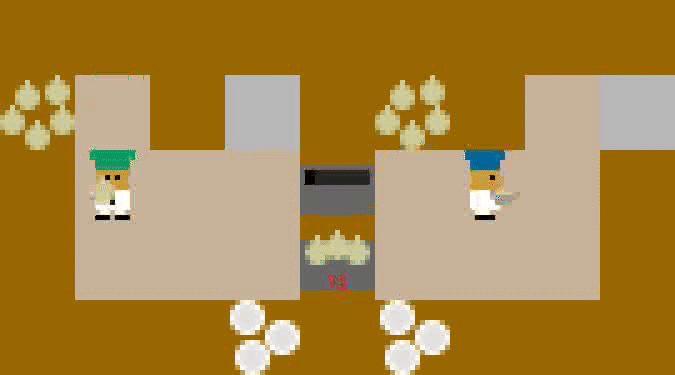
\includegraphics[trim=0cm -0.5cm 0cm -0.5cm, clip, width=0.9\linewidth]{figures/overcooked.png}
    \caption[Capture d'écran de l'environnement Overcooked-AI]{Capture d'écran de l'environnement Overcooked-AI : deux agents (chefs cuisiniers) doivent collaborer pour préparer et servir efficacement des soupes à l'oignon. Le processus consiste à prélever trois oignons (un à la fois) dans le distributeur, à les placer dans une marmite, à attendre que la soupe cuise, à récupérer un plat propre, à dresser la soupe et à la livrer au comptoir de service. La disposition de la cuisine comprend des obstacles et des passages étroits, ce qui oblige les agents à coordonner leurs mouvements pour éviter les collisions et optimiser l'accomplissement des tâches.}
    \label{fig:overcooked}
\end{figure}


\subsection{Configuration matérielle}

Toutes les expériences ont été menées sur un cluster académique haute performance, avec des nœuds GPU (NVIDIA A100, V100 et AMD MI210). Chaque configuration algorithme-environnement a été exécutée 5 fois en parallèle pour assurer des résultats fiables.
Les hyperparamètres~\hyperref[fn:github]{\footnotemark[1]} (taux d'apprentissage, facteurs d'actualisation, taux d'exploration) proviennent soit des banques de MARLlib, soit d’une recherche sur grille réalisée via \textit{Optuna}~\cite{akiba2019optuna}.

\subsection{Métriques d'évaluation et protocole}

L'évaluation prend en compte l'efficacité des politiques et l'impact des spécifications organisationnelles en reposant sur les métriques suivantes :
%
i) \textbf{Récompense Cumulative} : Mesure l'efficacité de la politique dans l'atteinte des objectifs de l'environnement
; \quad
ii) \textbf{Écart-type de la Récompense} : Reflète la stabilité des politiques apprises au cours des épisodes
; \quad
iii) \textbf{Taux de Convergence} : Indique la rapidité avec laquelle les politiques atteignent une performance stable
; \quad
iv) \textbf{Taux de Violation des Contraintes} : Évalue le respect des contraintes organisationnelles par la politique, ce qui est crucial pour la sécurité
; \quad
v) \textbf{Score de Cohérence} : Mesure l'alignement entre les comportements appris et les spécifications organisationnelles
; \quad
vi) \textbf{Score de Robustesse} : Évalue la capacité des agents à maintenir leur performance face à une série de scénarios difficiles
; \quad
vii) \textbf{Niveau d'Adéquation Organisationnelle} : Quantifie l'adéquation organisationnelle avec TEMM.

Notre protocole compare le \textit{Baseline de Référence} (RB) sans contraintes organisationnelles au \textit{Baseline Organisé} (OB) utilisant MOISE+MARL.
Pour le RB, nous utilisons MMA pour entraîner les agents dans chaque environnement (jusqu'à convergence ou limite d'épisodes) sans appliquer de spécifications organisationnelles, puis nous sélectionnons l'algorithme obtenant la Récompense Cumulative maximale.
Pour l'OB, nous réinitialisons environnements et agents, appliquons via MMA des spécifications prédéfinies (chaque agent se voit attribuer un rôle) et ré-entraînons ces agents avec l'algorithme le plus performant du RB. Les métriques permettent alors des comparaisons.
%
Nous évaluons l'impact de MOISE+MARL en vérifiant si les comportements des agents s'alignent avec les rôles définis (à l'aide de l'Écart-type de Récompense, du Taux de Convergence et du Score de Robustesse). Une différence significative du Niveau d'Adéquation Organisationnelle entre RB et OB, et une corrélation entre les rôles et ce niveau, confirmera l'efficacité du cadre.
Enfin, nous comparons MOISE+MARL à AGR+MARL (qui ne considère que les rôles) pour évaluer l'importance des missions.

\section{Résultats}
\label{sec:results}

Cette section discute des résultats obtenus sur les quatre environnements.

\begin{table*}[h!]
    \centering
    \caption{Résultats détaillés pour chaque environnement et algorithme favorisé, pour le RB et l'OB.}
    \label{tab:detailed_results}
    \footnotesize
    \renewcommand{\arraystretch}{1.2}
    \begin{tabular}{p{1.8cm}p{1.1cm}p{.5cm}p{0.7cm}p{0.7cm}p{0.7cm}p{0.7cm}p{0.7cm}p{0.7cm}p{0.7cm}}
        \hline
        \textbf{Env.} & \textbf{Alg.} & \textbf{Spec. Org.} & \textbf{Récom. Cum.} & \textbf{Écart-Type} & \textbf{Taux Conv.} & \textbf{Taux Viol.} & \textbf{Score Cohé.} & \textbf{Score Rob.} & \textbf{Niv. Adéq.} \\ \hline
        Predator-Prey & MADDPG        &                     & 200.1                & 21.5                & 0.65                & 12.3\%              & -                    & 0.65                & 0.43                \\
        Predator-Prey & MADDPG        & Oui                 & 245.8                & 15.2                & 0.85                & 0.0\%               & 0.81                 & 0.83                & 0.87                \\
        Overcooked-AI & MAPPO         &                     & 348.2                & 15.6                & 0.75                & 7.1\%               & -                    & 0.71                & 0.48                \\
        Overcooked-AI & MAPPO         & Oui                 & 391.2                & 10.4                & 0.92                & 0.0\%               & 0.89                 & 0.89                & 0.91                \\
        Warehouse M.  & Q-Mix         &                     & 257.4                & 18.9                & 0.74                & 7.8\%               & -                    & 0.68                & 0.50                \\
        Warehouse M.  & Q-Mix         & Oui                 & 307.1                & 13.8                & 0.88                & 0.0\%               & 0.88                 & 0.86                & 0.90                \\
        Cyber-Defense & COMA          &                     & 162.4                & 17.3                & 0.70                & 12.2\%              & -                    & 0.67                & 0.45                \\
        Cyber-Defense & COMA          & Oui                 & 188.9                & 11.2                & 0.86                & 0.0\%               & 0.76                 & 0.80                & 0.83                \\ \hline
    \end{tabular}
\end{table*}

\subsection{Adéquation organisationnelle quantitative et cohérence}

\noindent
Comme l'illustre le \autoref{tab:detailed_results}, l'adéquation organisationnelle est systématiquement plus élevée dans l'OB, confirmant que MOISE+MARL aligne efficacement le comportement des agents sur les spécifications organisationnelles.
Par exemple, dans \textbf{Predator-Prey} avec \textbf{MADDPG}, l'OB atteint un niveau d'adéquation de 0.87 (soit +49\% par rapport aux 0.43 du RB), tandis que dans \textbf{Overcooked-AI} avec \textbf{MAPPO}, on observe 0.91 (+89\%). Même constat pour \textbf{Warehouse Management} avec \textbf{Q-Mix}, où l'adéquation passe de 0.50 (RB) à 0.90 (OB).

\medskip
\noindent
De façon générale, contraindre les agents par des spécifications organisationnelles diminue la déviation de récompense et accélère la convergence, indiquant un impact notable sur leur comportement. Nous avons observé manuellement, notamment dans \textbf{Predator-Prey}, que les politiques entraînées correspondent bien à une organisation structurelle et fonctionnelle implicite.

\medskip
\noindent
Le \textbf{score de cohérence} demeure également élevé (jusqu’à 0.76 dans le contexte bruité de \textbf{Cyber-Defense}), montrant que, malgré les perturbations, les spécifications organisationnelles inférées sont proches de celles appliquées.

\subsection{Element d'explicabilités : exemple de Overcooked-AI}

Nous avons appliqué MMA ainsi que la méthode TEMM pour générer une quinzaine de trajectoires d'agents entraînés avec \textbf{MAPPO} dans \textbf{Overcooked-AI}, selon les spécifications organisationnelles suivantes pour les deux agents cuisiniers :
%
\begin{itemize}
    \item Rôle "Polyvalent" : "si l'agent a un bol et voit un pot plein dans une case adjacente, il doit interagir avec le pot pour récupérer la soupe" et "si l'agent a une soupe et voit le comptoir de service dans une case adjacente, il doit interagir avec le comptoir pour livrer la soupe"
    \item Objectif "Tenir bol de soupe" : "tient un bol de soupe"
\end{itemize}

Après application de TEMM, nous avons obtenu un score d'adéquation organisationnel de 0.87, indiquant des comportements d'agents entrainés assez réguliers même en dehors des comportements contraints. TEMM permet d'inferrer de nouvelles règles et observations sous forme vectorielle (avec une distance euclidienne). Après analyse, ces règles peuvent être retranscrites en langage naturel et confirment que les agents ont complété les règles initiales par d'autres qui semblent les amener à atteindre l'objectif fixé. Par exemple~:
%
\begin{itemize}
    \item Règles RAG : "si l'agent n'a pas de bol et voit un bol vide dans une case adjacente, il doit interagir avec le bol pour le ramasser" et "si l'agent n'a pas d'oignon et voit un oignon dans une case adjacente, il doit interagir avec l'oignon pour le ramasser"
    \item Observations GRG : "Cuisson en cours" : "voit un pot en train de cuire"
\end{itemize}

Pour obtenir une meilleure représentation des trajectoires et des centroïdes, notre implémentation de TEMM génère également des figures telles que des dendrogrammes ou des visualisations en deux dimensions via une ACP. Dans ces deux visualisations, on remarque la similarité des comportements entre les deux agents, ce qui est cohérent avec le fait qu'ils partagent le même rôle et objectif. Par ailleurs, bien que l'entraînement aurait pu conduire à des comportements divergents, on observe tout de même une conservation du comportement attendu, probablement due à la symétrie spatiale de l'environnement utilisé. Cela se traduit par deux clusters (un pour chaque agent) qui, bien que distincts, sont regroupés dans le même macro-cluster (\autoref{fig:overcooked_dendrogram}) représentant le rôle "Polyvalent" enrichi des règles post-entraînement. Ce phénomène peut également être observé dans la visualisation en deux dimensions (\autoref{fig:overcooked_pca}), où les trajectoires des deux agents sont en fait le symétrique l'une de l'autre, ce qui est cohérent avec la nature symétrique de l'environnement spatial d'Overcooked-AI.

\begin{figure}[h!]
    \centering
    \includegraphics[trim=0cm 1cm 0cm 0.9cm, clip, width=0.8\linewidth]{figures/overcooked_figures/full_dendrogram.pdf}
    \caption{Dendrogramme des trajectoires de transition dans Overcooked-AI}
    \label{fig:overcooked_dendrogram}
\end{figure}

\begin{figure}[h!]
    \centering
    \includegraphics[trim=0cm 1cm 0cm 0.9cm, clip, width=0.8\linewidth]{figures/overcooked_figures/transition_pca.pdf}
    \caption{PCA des trajectoires de transition dans Overcooked-AI}
    \label{fig:overcooked_pca}
\end{figure}


\subsection{Performance et stabilité selon les algorithmes}

Les résultats indiquent que les algorithmes basés sur la politique et les algorithmes acteur-critique, tels que \textbf{MADDPG} et \textbf{MAPPO}, bénéficient considérablement du cadre MOISE+MARL, notamment en termes de cohérence et de stabilité. Par exemple, dans l'environnement \textbf{Overcooked-AI}, \textbf{MAPPO} a vu son écart-type de récompense passer de 15.6 (RB) à 10.4 (OB), reflétant une politique plus stable avec moins de fluctuations comportementales. De même, \textbf{MADDPG} dans \textbf{Predator-Prey} a montré une diminution similaire, passant de 21.5 en RB à 15.2 en OB, indiquant une fiabilité accrue.

En revanche, les algorithmes basés sur la valeur, comme \textbf{Q-Mix}, ont maintenu une haute performance en récompense cumulative, mais ont affiché une variabilité plus importante en termes de cohérence. Par exemple, dans l'environnement \textbf{Warehouse Management}, \textbf{Q-Mix} a atteint un écart-type de récompense de 13.8 en OB, soit une amélioration notable par rapport aux 18.9 en RB, mais toujours supérieur à la stabilité observée dans les algorithmes basés sur la politique. Cela suggère que, bien que \textbf{Q-Mix} soit efficace pour atteindre les objectifs de la tâche, il pourrait nécessiter un ajustement supplémentaire pour les rôles avec MOISE+MARL afin d'améliorer la cohérence.

\subsection{Impact des contraintes organisationnelles sur la convergence, la robustesse et le taux de violation des politiques}

L'application des contraintes organisationnelles a permis d'accélérer les taux de convergence dans tous les environnements. Dans l'environnement \textbf{Cyber-Defense}, \textbf{COMA} avec MOISE+MARL a convergé à un taux de 0.86, contre 0.70 en RB. Des tendances similaires ont été observées dans l'environnement \textbf{Warehouse Management} avec \textbf{Q-Mix}, qui est passé de 0.74 en RB à 0.88 en OB. Cette convergence accélérée est attribuée à un espace de recherche plus contraint par les rôles et objectifs.

En outre, nous avons observé que les taux de violation des contraintes étaient systématiquement plus élevés lorsque les contraintes organisationnelles étaient définies avec une rigidité de contrainte plus faible. Dans l'environnement \textbf{Overcooked-AI}, \textbf{MAPPO} a enregistré un taux de violation nul avec une rigidité de contrainte de 1, contre 7.1\% avec une rigidité de 0. De même, dans \textbf{Warehouse Management}, \textbf{Q-Mix} a effectivement vu le taux de violation passer de 7.8\% à zéro quand la rigidité est à 1.

De plus, nous avons observé une amélioration constante de la robustesse lorsque les spécifications organisationnelles étaient appliquées aux agents. Par exemple, \textbf{MADDPG} dans \textbf{Predator-Prey} et \textbf{MAPPO} dans \textbf{Overcooked-AI} ont obtenu des scores de cohérence élevés, respectivement 0.81 et 0.89, indiquant que les agents suivaient de près les rôles inférés. La robustesse s'est également améliorée, avec \textbf{MAPPO} dans \textbf{Overcooked-AI} atteignant un score de robustesse de 0.89, contre 0.71 en RB, soulignant une meilleure résilience face aux perturbations.

Cependant, un biais potentiel peut être souligné : les spécifications organisationnelles ont été conçues pour englober toutes les observations, évitant ainsi les situations nouvelles non gérées.

\subsection{Comparaison entre MOISE+MARL et AGR+MARL}

\begin{table}[h!]
    \centering
    \caption{Comparaison de la performance entre MOISE+MARL et AGR+MARL.}
    \label{tab:ablation_study}
    \footnotesize
    \renewcommand{\arraystretch}{1.1}
    \begin{tabular}{p{2.1cm}p{0.5cm}p{0.7cm}p{0.7cm}p{0.6cm}p{0.9cm}}
        \hline
        \textbf{Framework} & \textbf{Env.} & \textbf{Taux Conv.} & \textbf{Score Rob.} & \textbf{Niv. Adéq.} & \textbf{Récom. Cum.} \\ \hline
        MOISE+MARL         & PP            & 0.85                & 0.83                & 0.87                & 245.8                \\
        AGR+MARL           & PP            & 0.75                & 0.69                & 0.56                & 208.4                \\
        MOISE+MARL         & OA            & 0.92                & 0.89                & 0.91                & 391.2                \\
        AGR+MARL           & OA            & 0.82                & 0.75                & 0.58                & 348.9                \\
        MOISE+MARL         & WM            & 0.88                & 0.86                & 0.90                & 307.1                \\
        AGR+MARL           & WM            & 0.76                & 0.72                & 0.61                & 278.6                \\ \hline
    \end{tabular}
\end{table}

\paragraph{Impact des objectifs intermédiaires}
Le \autoref{tab:ablation_study} met en lumière l’effet de ces objectifs dans MOISE+MARL. Dans \textbf{Overcooked-AI}, \textbf{MAPPO} obtient une récompense cumulative de 391.2 et une adéquation organisationnelle de 0.91, soit 33\% de plus qu’AGR+MARL (0.58). Dans \textbf{Warehouse Management}, \textbf{Q-Mix} sous MOISE+MARL atteint 307.1 de récompense (contre 278.6 pour AGR+MARL) et un score de robustesse supérieur (0.86 vs 0.72).

Ces résultats soulignent l’importance des objectifs intermédiaires pour des comportements plus stables et mieux orientés vers l’objectif. MOISE+MARL surpasse ainsi AGR+MARL en récompense, robustesse et adéquation organisationnelle dans \textbf{Predator-Prey}, \textbf{Warehouse Management} et \textbf{Overcooked-AI}.
%
Enfin, l’augmentation du nombre de contraintes organisationnelles accroît quasi linéairement la durée d’entraînement, d’après nos premiers résultats~\hyperref[fn:github]{\footnotemark[1]}.

\section{Conclusion et travaux futurs}
\label{sec:discussion_conclusion_future_work}

Nous avons introduit le cadre MOISE+MARL, qui couple un modèle organisationnel explicite au MARL afin d'améliorer le contrôle et l'explicabilité des politiques multi-agent. Les expérimentations démontrent une convergence plus rapide, une stabilité accrue et une cohérence renforcée entre les comportements appris et les spécifications organisationnelles, qu'elles soient définies ou inférées.

Deux axes de recherche se dessinent pour la suite : d'une part, l'exploration de nouvelles approches visant à automatiser davantage la méthode TEMM, notamment par l'intégration de modèles de langage de grande taille (\textit{Large Language Models}), et d'autre part, l'amélioration de la scalabilité de TEMM ainsi que le développement de solutions pour réduire le surcoût computationnel. Ces perspectives devraient permettre une meilleure intégration de l'organisation dans le MARL, renforçant la robustesse, la sûreté et l'explicabilité des agents dans des systèmes réels.

\newpage
%\nocite{*}
\bibliography{references}

\bigskip

% Pour afficher les r{\'e}sum{\'e}s anglais et fran{\c c}ais
\setotherabstracts

\end{document}




